%Version 3.1 December 2024
\documentclass[pdflatex,sn-apa]{sn-jnl}

\usepackage{graphicx}
\usepackage{booktabs}
\usepackage{tabularx}
\usepackage{array}
\usepackage{longtable}
\usepackage{amsmath,amssymb,amsfonts}
\usepackage{xcolor}
\usepackage{textcomp}

\raggedbottom

\newcommand{\toolkit}{PPS Toolkit}
\newcommand{\code}[1]{\texttt{#1}}

\begin{document}

\title[PPS Toolkit suite for audio-tactile PPS experiments]{PPS Toolkit: A suite for designing, running, and recreating audio-tactile peripersonal-space experiments}

\author*[1]{\fnm{George} \sur{Fejer}}\email{author.email@example.com}

\affil*[1]{\orgname{Institution to be added}, \orgaddress{\country{Country to be added}}}

\abstract{Researchers use audio-tactile peripersonal-space (PPS) experiments to estimate how quickly an approaching sound speeds tactile responses near the body. To run one such task, an experimenter must fix the auditory waveform, the level and gain law that imply distance, the looming trajectory, the body-relative direction, the tactile site and its intensity calibration, the baseline and control conditions, the randomization, the response rule, the timing validation, and the model that summarizes distance-dependent facilitation. Each choice changes what the experiment measures, yet most studies bury these choices in custom scripts, filenames, and lab notebooks, which leaves later readers unable to replicate, reuse, or even fully report the design. We present \toolkit{}, an open-source suite that walks a researcher through these decisions and then runs the resulting task. The dashboard breaks the experiment into auditable segments: the researcher selects a study profile, builds the auditory source, assembles the within-trial sequence, generates tactile and baseline trials, sets the repetition pool, reviews the block-level randomization, and prepares the native runner that delivers synchronized playback and logs responses. At each step the suite writes a manifest, hashes the generated assets, keeps reusable profiles separate from participant outputs, and labels its evidence by tier, separating software timing from digital audio, electrical loopback, and perceptual tactile calibration. We contribute a design-decision evidence matrix that links every literature-bearing control in the interface to the methodological variation it governs in the PPS literature: burst-train versus smooth looming sounds, loudness and gain policies, fixed-distance and tactile-only baselines, near-field spatial rendering with SOFA/HRTF resources, tactile threshold calibration, missed-trial safeguards, and exploratory model fitting. The suite does not impose one canonical PPS paradigm. It makes the heterogeneous decisions behind a PPS task explicit enough that another laboratory can design, run, reproduce, critique, and extend the experiment.}

\keywords{peripersonal space, audio-tactile integration, behavioral methods, spatial audio, HRTF, tactile calibration, open-source software}

\maketitle

\section{Introduction}

In an audio-tactile PPS task, the participant responds as fast as possible to a tactile target while a task-irrelevant sound approaches, recedes, or holds at a controlled distance. When the sound reaches a position close enough to the body to enter a multisensory action space, tactile responses speed up, and the distance at which that speed-up appears indexes the boundary of peripersonal space \citep{Canzoneri2012}.

The field has since carried this logic into front, rear, left, and right spaces \citep{Matsuda2021,Amiel2025,Teraoka2024}, into walking and action remapping \citep{Noel2015}, into rough and affective sounds \citep{Taffou2021,Bahadori2021}, and onto smartphones that deliver synchronized audio-tactile stimulation \citep{Roussel2025}. Each variant answers a different question, and each changes the apparatus needed to run it.

That range is a strength, but it creates a problem for anyone who actually has to build and run one of these tasks. Two studies that both call themselves ``audio-tactile PPS'' can differ in the waveform that signals motion, the gain law that implies distance, the spatial path, the body-centered coordinate frame, the tactile site and how it is stimulated, the baseline used for correction, the proportion of catch trials, the response device, and the model that estimates the boundary or gradient. These are not interchangeable settings. They determine what reaction-time curve the experiment can produce.

The field already knows the cost of leaving them implicit. A methodological critique and meta-analysis found mixed evidence for near-sound tactile facilitation and traced much of the inconsistency to control conditions, temporal expectancy, response probability, trial counts, and flexible analysis choices \citep{Holmes2020}. A design proposal then showed that a fixed-distance baseline, chosen with sound-propagation properties in mind, sharpens what a dynamic audio-tactile effect can mean \citep{Hobeika2019}. Neither paper diminishes the paradigm. Both show that when a researcher cannot recover exactly how a PPS task was run, the resulting estimate is hard to trust.

We built \toolkit{} to keep those running decisions visible across the whole lifecycle of a PPS experiment. The suite is a Windows-ready, open-source environment in which a researcher builds a new audio-tactile PPS task, opens a published paradigm as an inspectable profile, renders the stimuli, runs the synchronized session, and reviews the validation and analysis artifacts, all without editing scripts.

The suite couples an HTML design dashboard, a registry of published profiles, a renderer that records SOFA/HRTF and 3D Tune-In-compatible spatialization metadata, a native Focus Mode runner that plays multichannel audio in sync and logs responses, and post-run analysis that keeps exploratory plots apart from confirmatory inference. Following the pattern of Behavior Research Methods software papers and experiment-builder reports \citep{AnwylIrvine2018,Peirce2019,Otto2023}, the contribution is a working instrument: a tool that surfaces the decisions a PPS task usually hides.

This manuscript does three things. It documents why the toolkit exposes the controls it does, using a structured evidence matrix rather than a formal meta-analysis. It describes the workflow and architecture that turn PPS design decisions and published-profile recreations into runnable audio-tactile trials. And it draws conservative validation boundaries, separating software and digital-audio evidence from electrical loopback evidence and from tactile perception. We claim no participant-level effect here. We treat the pilot observation that tactile miss rates can climb during long sessions after threshold calibration as design motivation only, until traceable run artifacts back it.

\section{Contribution and Journal Fit}

This manuscript belongs in Behavior Research Methods because it builds a method rather than reports a new PPS effect. The contribution is a reusable research instrument: a stimulus-development workflow, a trial-assembly interface, a published-profile recreation layer, a native reaction-time runner, and a matched set of analysis and validation artifacts.

Comparable behavioral software papers ask how a tool lowers technical barriers while it preserves timing, extensibility, and reproducibility \citep{AnwylIrvine2018,Peirce2019,Akam2022,Otto2023}. By that standard the test is not whether we prove a new boundary estimate. It is whether we show what the software lets a researcher specify, recreate, run, and validate, what it records for reuse, and which claims fall outside the software evidence.

\toolkit{} is also narrower than a general experiment builder. Gorilla and PsychoPy run broad classes of behavioral experiments \citep{AnwylIrvine2018,Peirce2019}; pyControl and related systems give flexible hardware control and task logic \citep{Akam2022}. \toolkit{} instead handles one hard corner of that space: an audio-tactile PPS session in which auditory motion, tactile timing, baseline logic, multichannel output, response logging, and spatial rendering must all line up before a single trial is valid. That demand is why we segment the interface. Each segment is a decision that running a PPS task forces on the experimenter, and that a custom script, a folder of WAV files, or a post-hoc notebook would otherwise hide.

A set of same-journal comparators shaped how we wrote this paper. Table~\ref{tab:brm-comparators} lists the article models we drew on, and \code{brm\_comparator\_articles.csv} stores the source audit. A recommendation ledger in \code{brm\_recommended\_article\_models.csv} records which BRM papers sit closest to \toolkit{} and what each one contributes to the draft. We do not imitate any single paper. We follow the recurring BRM pattern: state the barrier, show the tool, walk through a runnable example, give validation evidence, and mark the reuse boundaries.

\begin{table}[t]
\caption{Behavior Research Methods comparator articles used as style models.}
\label{tab:brm-comparators}
\footnotesize
\begin{tabularx}{\textwidth}{>{\raggedright\arraybackslash}p{0.20\textwidth} >{\raggedright\arraybackslash}X >{\raggedright\arraybackslash}p{0.30\textwidth}}
\toprule
Comparator cluster & Style lesson & PPS Toolkit implication \\
\midrule
General experiment builders & Gorilla, PsychoPy2, lab.js, OpenSesame, and PsyToolkit foreground usable tool workflows, graphical/scriptable access, timing-sensitive tasks, open materials, and examples \citep{AnwylIrvine2018,Peirce2019,Henninger2021,Mathot2011,Stoet2010}. & Present PPS Toolkit as an executable suite, not as a claim about a new PPS effect. \\
Hosting and sharing workflows & Open Lab and lab.js emphasize deployment, sharing, editable reuse, and transparent archiving while noting platform boundaries \citep{Shevchenko2022,Henninger2021}. & Separate hosted/static profile inspection from local native acquisition and participant outputs. \\
Specialized domain toolboxes & Vizard, virtual-navigation, broad behavioral-control, and immersive threat-avoidance toolboxes show design objectives, supported hardware boundaries, standardized outputs, and concrete examples \citep{Schuetz2022,AlsburyNealy2021,Otto2023,Brookes2023}. & Keep PPS-specific controls visible: auditory motion, SOA/tactile timing, baselines, HRTFs, runner route, and output artifacts. \\
Multimodal sensory and calibration suites & Browser tactile delivery, mobile psychophysics, cognitive-hearing extensions, eye-tracker toolboxes, adaptive calibration extensions, low-cost device evaluations, and mouse-tracking packages show how BRM papers document calibration/setup interfaces, synchronous I/O, device limits, and route suitability \citep{Hirst2026,Inuggi2024,Sulas2022,Niehorster2020,Niehorster2024Adaptive,Gibaldi2016,Kieslich2017}. & Present PPS Toolkit as a route-aware suite whose GUI, runner, validation artifacts, and analysis outputs must be reported together. \\
Analysis handoff and interoperability & Analysis toolkits and cross-platform frameworks show how raw event streams, visualization, statistical comparison, and external-tool boundaries can be made legible without turning exploratory outputs into confirmed effects \citep{Kieslich2017,Ghose2020,Henninger2016}. & Keep the native runner, LSL/LabRecorder route, generated manifests, and instant-analysis outputs explicitly separated by evidence role. \\
Timing and validation exemplars & Timing-comparison and simulation papers separate usability from route-specific timing evidence and encourage automated checks before participant interpretation \citep{Bridges2020,DeLeeuw2015,DeLeeuw2022}. & Report software, digital audio, electrical loopback, and perceptual tactile evidence as distinct layers. \\
\bottomrule
\end{tabularx}
\end{table}

The paper delivers three reusable products. The first is the design-run-recreation suite itself, covering new-study construction, published-profile recreation, native acquisition, validation evidence, and exploratory analysis review. The second is a design-decision evidence matrix that maps each visible GUI and runner choice to the methodological variation it controls in the PPS literature. The third is a reporting template: the manuscript keeps reusable profiles, local generated assets, participant outputs, timing evidence, tactile-perception evidence, and exploratory analysis as distinct categories a reader can cite. This responds to a growing concern that research assets can exist on paper yet still resist execution, inspection, or computational reuse \citep{Ellis2024}.

\subsection{Tutorial Use of the Manuscript and Source Package}

We wrote the article to serve as a tutorial and audit guide, not only as a software announcement. Table~\ref{tab:reader-guide} maps the questions a reader brings to the manuscript sections and source files that answer them. The organization follows the practical pattern of behavioral software papers: describe the tool, show how task logic becomes executable, identify the evidence a timing-sensitive claim needs, and make the reusable materials easy to inspect \citep{AnwylIrvine2018,Peirce2019,Akam2022,DeLeeuw2022}.

\begin{table}[t]
\caption{Reader guide for using the manuscript and source package.}
\label{tab:reader-guide}
\footnotesize
\begin{tabularx}{\textwidth}{>{\raggedright\arraybackslash}p{0.22\textwidth} >{\raggedright\arraybackslash}X >{\raggedright\arraybackslash}p{0.28\textwidth}}
\toprule
Reader question & Where to look & Practical use \\
\midrule
What design choices differ across PPS studies? & Design-decision evidence matrix, \code{evidence\_matrix.csv}, and \code{gui\_control\_coverage.csv}. & Identify which GUI and runner controls are scientific design decisions and which are operational controls. \\
How do I build a new PPS task? & PPS Toolkit overview and the design-run-recreation pathway. & Follow Segments 0--6 from profile/project selection through source generation, trial assembly, block review, and runner handoff. \\
How do I recreate a published paradigm? & Profiles and project registry, published-profile use case, and validation-evidence summary. & Inspect represented fields, missing apparatus details, local substitutions, verification status, and profile caveats before adapting the profile. \\
What evidence supports a run? & Technical method, validation/use cases, and archive-layer table. & Keep software schedules, digital audio evidence, electrical loopback evidence, and tactile perceptual evidence separate. \\
What should I report or share? & Reporting checklist, declarations, open-practices statement, and \code{submission\_readiness\_audit.md}. & Report provenance, hashes, baseline choices, response rules, validation tiers, analysis labels, and any artifacts that support the claims made. \\
\bottomrule
\end{tabularx}
\end{table}

\section{PPS Toolkit Overview}

\toolkit{} treats a PPS experiment as a chain of decisions, not a single monolithic script. Each dashboard segment owns a registry layer and writes the artifacts that the next segment consumes.

That structure follows the order in which a researcher actually reasons through a PPS task: choose the study profile, define the sound, lay out the within-trial sequence, set the tactile timing and controls, decide how many trials the design needs, inspect the block schedule, and hand the accepted design to the runner.

The workflow exposes seven segments, numbered 0 to 6. Segment 0 selects a bundled profile or creates a custom project. Segment 1 builds or imports the auditory ingredients. Segment 2 arranges those ingredients into within-trial sequence families. Segment 3 inserts the tactile cues and creates the baseline and catch files. Segment 4 expands the final trial assets into a repetition pool. Segment 5 distributes that pool into inspectable block CSV files. Segment 6 builds the participant-level block-order plans, prepares the output folder, and launches the native runner.

Figure~\ref{fig:workflow} lays out this segmented design and the archive layers it produces. The figure is schematic: it documents the workflow and the evidence boundary and makes no claim about behavioral validity.

\begin{figure}[t]
\centering
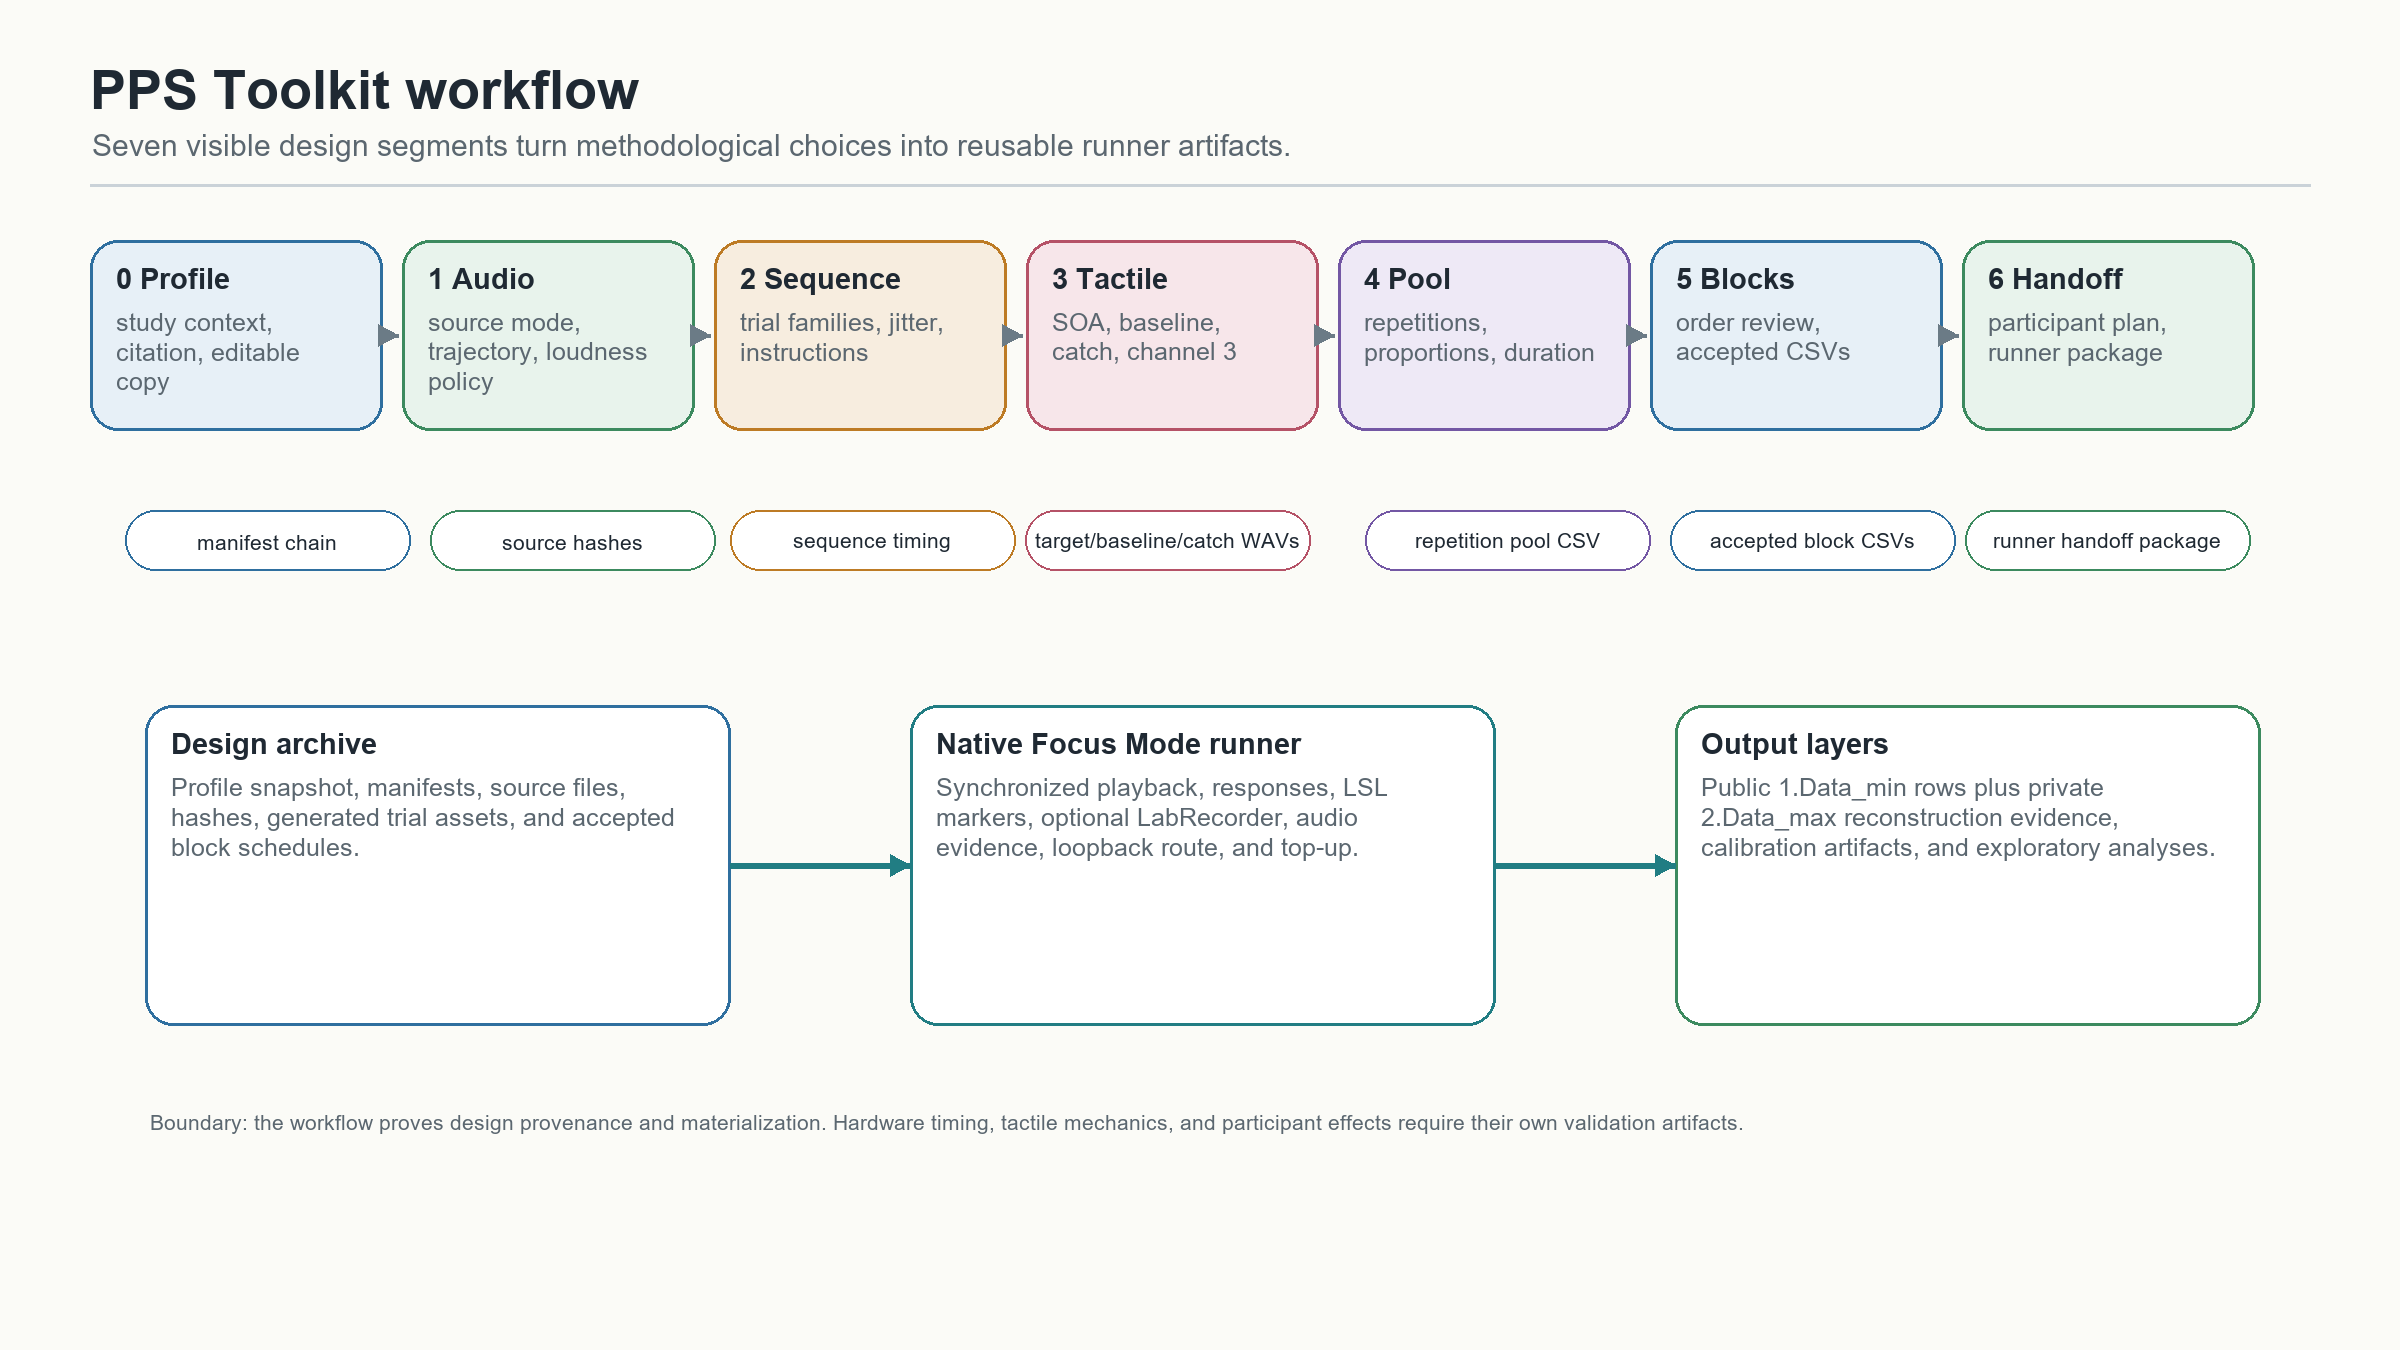
\includegraphics[width=\textwidth]{figures/figure1_workflow_segments.png}
\caption{PPS Toolkit workflow from profile selection to native runner handoff. The source-owned schematic shows how Segments 0--6 turn design choices into manifests, hashes, generated assets, accepted block schedules, runner packages, and output layers. It supports the suite-workflow claim, but it is not timing, tactile-mechanical, or participant-effect evidence.}
\label{fig:workflow}
\end{figure}

Each segment records the upstream manifest hash it consumed, so the suite can flag a stale downstream artifact instead of reusing it silently.

This segmentation is more than a user-interface preference. It is a reproducibility control. A PPS result turns on choices that are easy to lose after the fact: whether the sound was continuous or burst-like, whether an apparent baseline was tactile-only or stationary-auditory, whether catch trials reused the same auditory file without channel 3, whether randomization preserved trial-family order, or whether the runner raised tactile output after repeated misses. By making each choice visible and persistent, the toolkit converts the field's design heterogeneity into something a methods section can report.

Figure~\ref{fig:decision-map} maps the visible controls onto the PPS method decisions they encode. It separates a scientific design decision from ordinary interface mechanics and points the reader back to the editable source ledgers.

\begin{figure}[t]
\centering
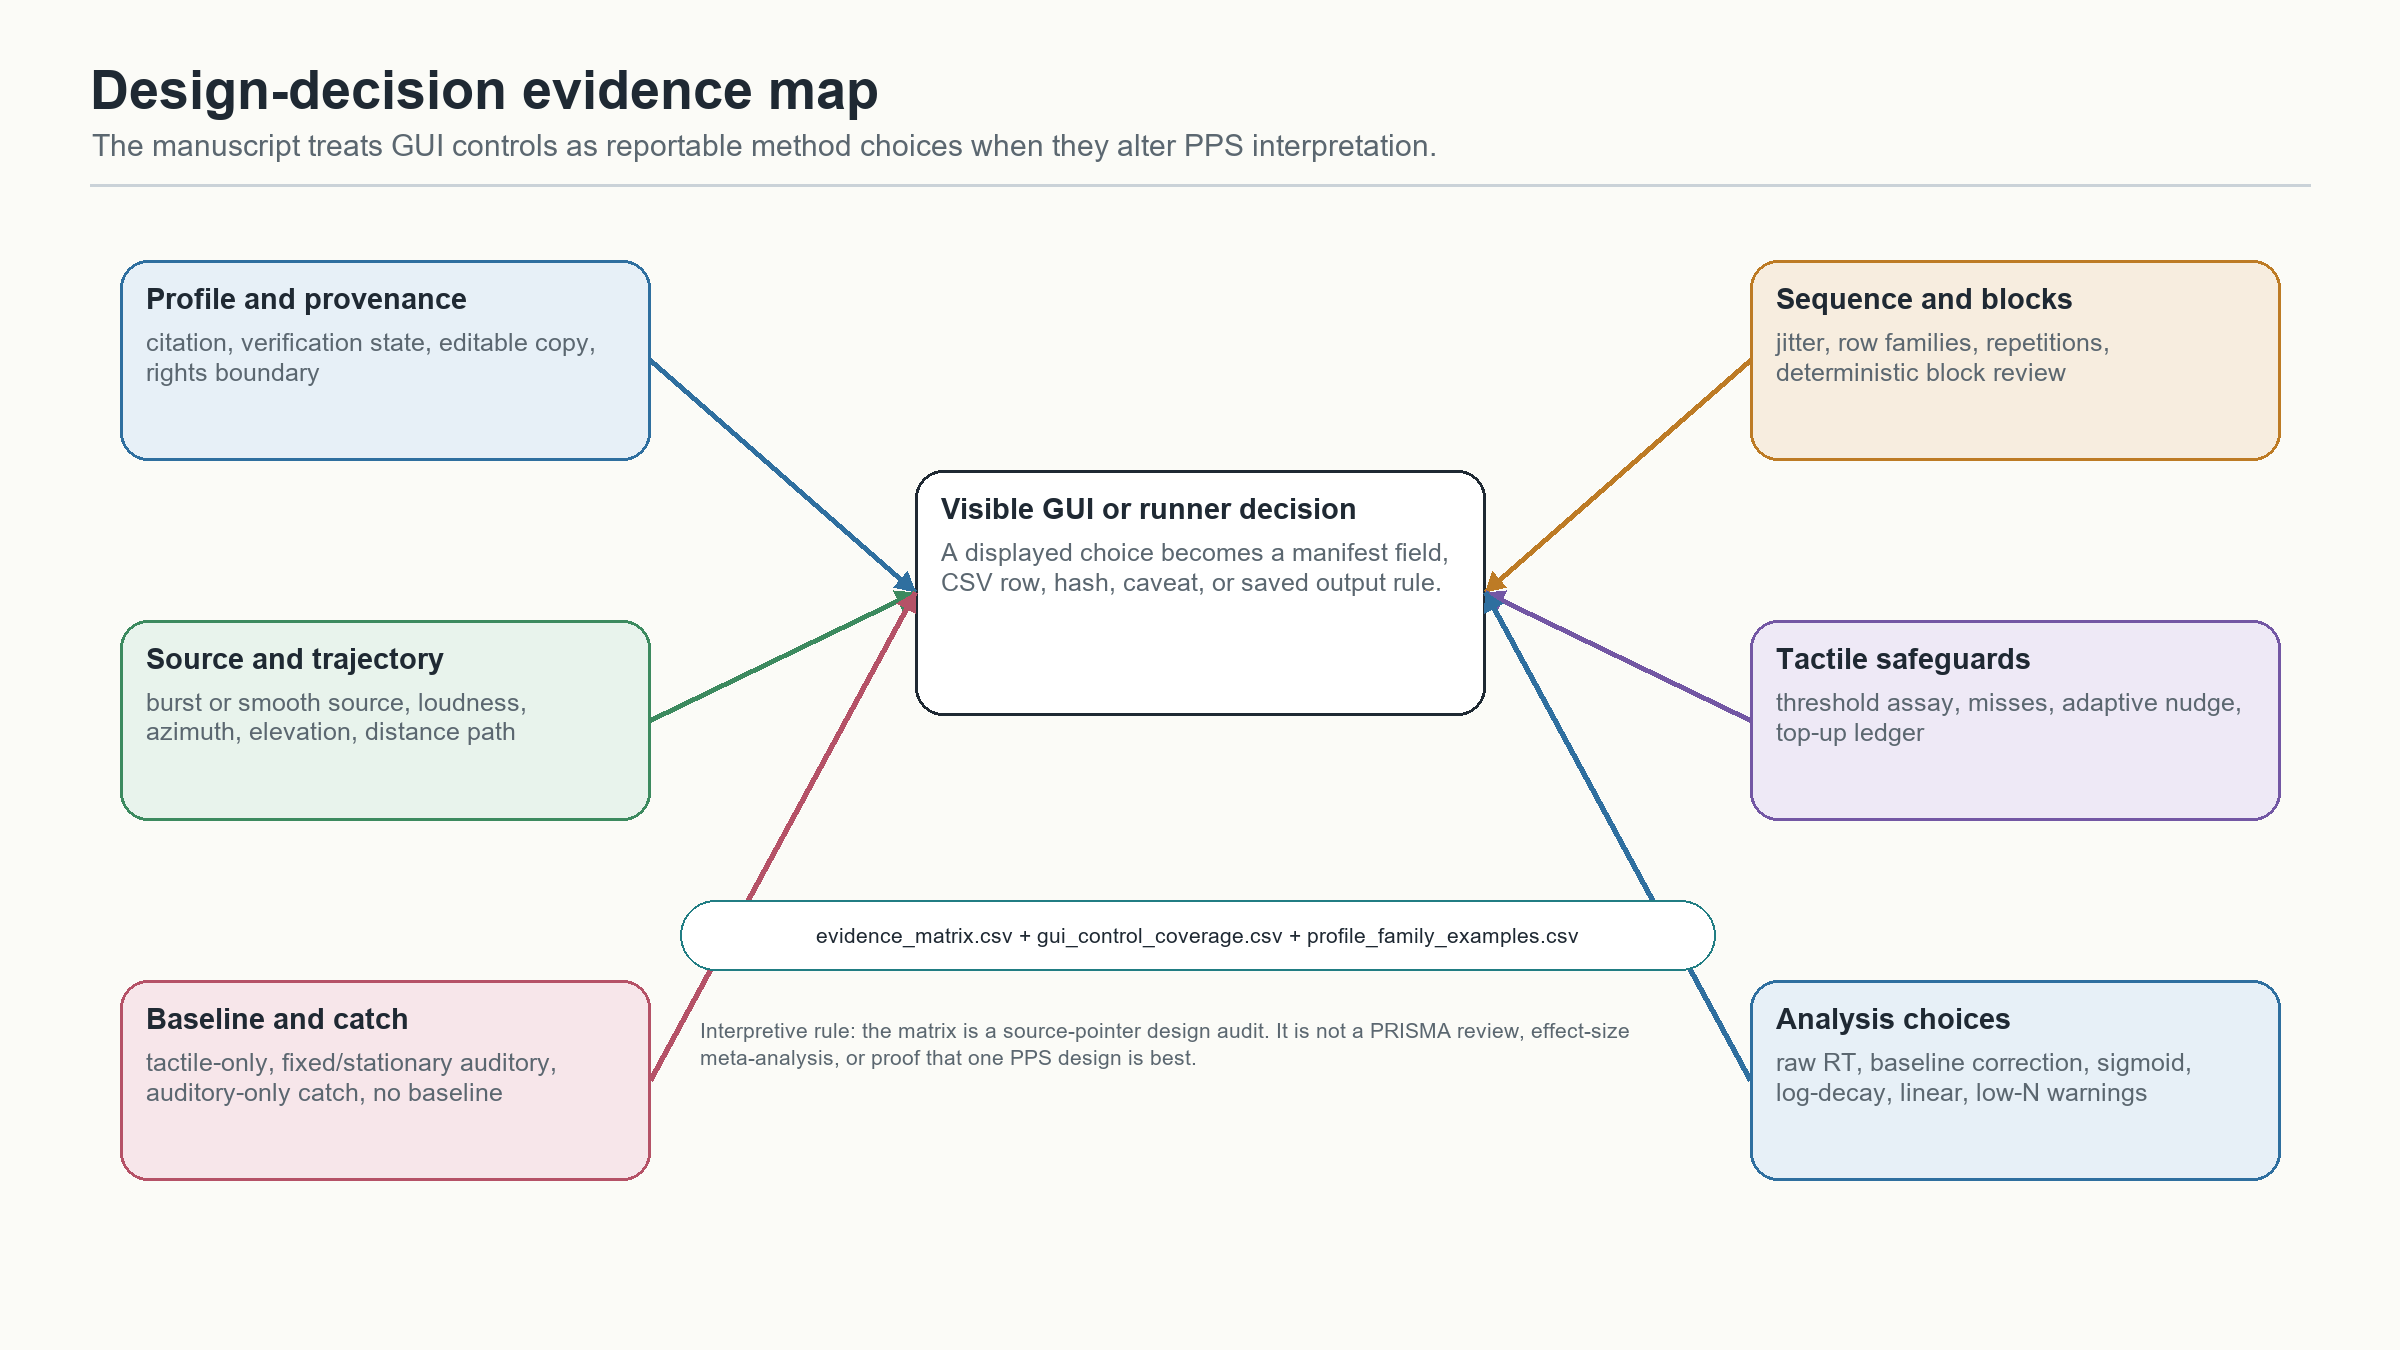
\includegraphics[width=\textwidth]{figures/figure2_design_decision_map.png}
\caption{Design-decision evidence map. Literature-bearing GUI and runner controls are grouped by the kind of PPS method choice they alter and are linked to editable source ledgers. The map is a source-pointer audit scaffold, not a PRISMA-style review or effect-size meta-analysis.}
\label{fig:decision-map}
\end{figure}

The visible \emph{Apply}, \emph{Bake}, \emph{Accept}, \emph{Prepare}, and \emph{Start Experiment Runner} actions are therefore part of the method. Each one is the moment a displayed choice becomes a durable artifact: a project registry entry, a source manifest, a generated WAV, a sequence manifest, a baseline/catch file set, a repetition-pool CSV, an accepted block schedule, a participant-order file, or a runner handoff package.

When an upstream decision changes, the suite marks the downstream products stale instead of reusing them. This follows a broader behavioral-software principle: an experiment builder should make task logic executable and inspectable \citep{AnwylIrvine2018,Akam2022}, and validation or simulation should catch a technical error before anyone interprets participant data \citep{DeLeeuw2022,Ellis2024}.

\subsection{Profiles and Project Registry}

Segment 0 sets the study context. Bundled profiles give a researcher a reusable starting point for published and laboratory paradigms, including a Study 5-style breathing workflow, a DynaSpace-inspired lateral variant, the Canzoneri dynamic-sound family, four-direction and front/rear profiles, smartphone and DynaSpace profiles, affective and rough-sound variants, and partial recreations of tool-use, walking, echolocation, wheelchair, and 3D/VR boundary paradigms.

Every profile carries a citation, a verification status, the fields it represents, and its caveats. A verified profile means we checked the fields the current toolkit represents against accessible methods or local reference materials. It does not mean the toolkit redistributes the original authors' sound files or reproduces every apparatus property.

A custom project writes its own local registry folder and manifests. The public repository deliberately leaves out local participant outputs, private generated assets, raw downloaded papers, local SOFA files, and unlicensed third-party stimuli. This boundary keeps the software reusable while it prevents a researcher from accidentally publishing data or assets that do not belong in a methods package.

The dashboard also keeps inspection, editing, and acquisition apart. A bundled profile opens in view mode, so a researcher can read its citations, paths, and previews before copying the design into an editable local project. Hosted and static pages preview a finished profile and export source-pointer randomization artifacts, but they never run a timing-sensitive trial or write a participant folder. This follows the same lesson as the general experiment builders: a graphical interface lowers barriers and improves reuse \citep{AnwylIrvine2018,Peirce2019}, but a reaction-time or audio-timing claim still has to be validated on the actual browser, operating system, audio route, and hardware that will run the study \citep{Bridges2020,Ellis2024}.

\subsection{Auditory Ingredients}

Segment 1 keeps source construction separate from trial scheduling. A researcher can generate a looming noise source, import a custom source for spatialization, or keep a custom audio clip such as an instruction or speech segment. Generated looming currently offers two source modes. \emph{Burst train} maps to the toolkit's DynaSpace-derived Gaussian burst-train profile; \emph{Smooth linear} maps to a continuous-noise profile.

The source-mode toggle exists because the field has never settled on one auditory source form. Canonical dynamic-sound tasks drove the approach with noise-like looming stimuli \citep{Canzoneri2012,Farne2002}, whereas recent mobile and DynaSpace workflows favor salient burst trains with validated phone timing \citep{Roussel2025}. Still other PPS work builds the manipulation from roughness, affective sounds, ecological sounds, or semantic sounds whose defensive or action-preparation value is the point \citep{Taffou2021,Bahadori2021}. The mode a researcher picks changes what the approaching sound means, so the toolkit asks for it explicitly.

Segment 1 also makes the researcher commit to a loudness contract rather than leave each source with an implicit gain. Sound level, direct-to-reverberant ratio, source spectrum, and source type all shape how far away a listener judges a sound to be \citep{Zahorik2002,Kolarik2015}. For nearby virtual sources, intensity can swamp subtler HRTF distance cues, and even the choice to normalize level becomes a cue in its own right \citep{Spagnol2017,Arend2021Level}. The toolkit therefore records the intended start and end SPL policy, the instruction offset, the peak ceiling, and whether each value is estimated or physically measured. The default hardware estimate is a convenience profile, not publication-grade acoustic calibration.

Segment 1 also records the source trajectory: start and end distance, azimuth, elevation, duration, hold periods, and the derived path and speed. The point is to preserve the body-relative frame the experiment depends on. Front, rear, left, and right approaches yield different PPS profiles \citep{Matsuda2021,Teraoka2024,Amiel2025}; walking and action remapping move the effective boundary \citep{Noel2015}; and VR/3D paradigms treat PPS as a volume rather than a single axis \citep{Lerner2021}. A file named \code{looming.wav} cannot carry any of that. The trajectory samples, the source hashes, and the renderer metadata are part of the stimulus.

Figure~\ref{fig:stimulus-alternatives} shows the three stimulus decisions that are easiest to conflate: source form, body-relative trajectory, and baseline/catch structure. PPS Toolkit stores them separately because each one changes the interpretation of an audio-tactile RT curve.

\begin{figure}[t]
\centering
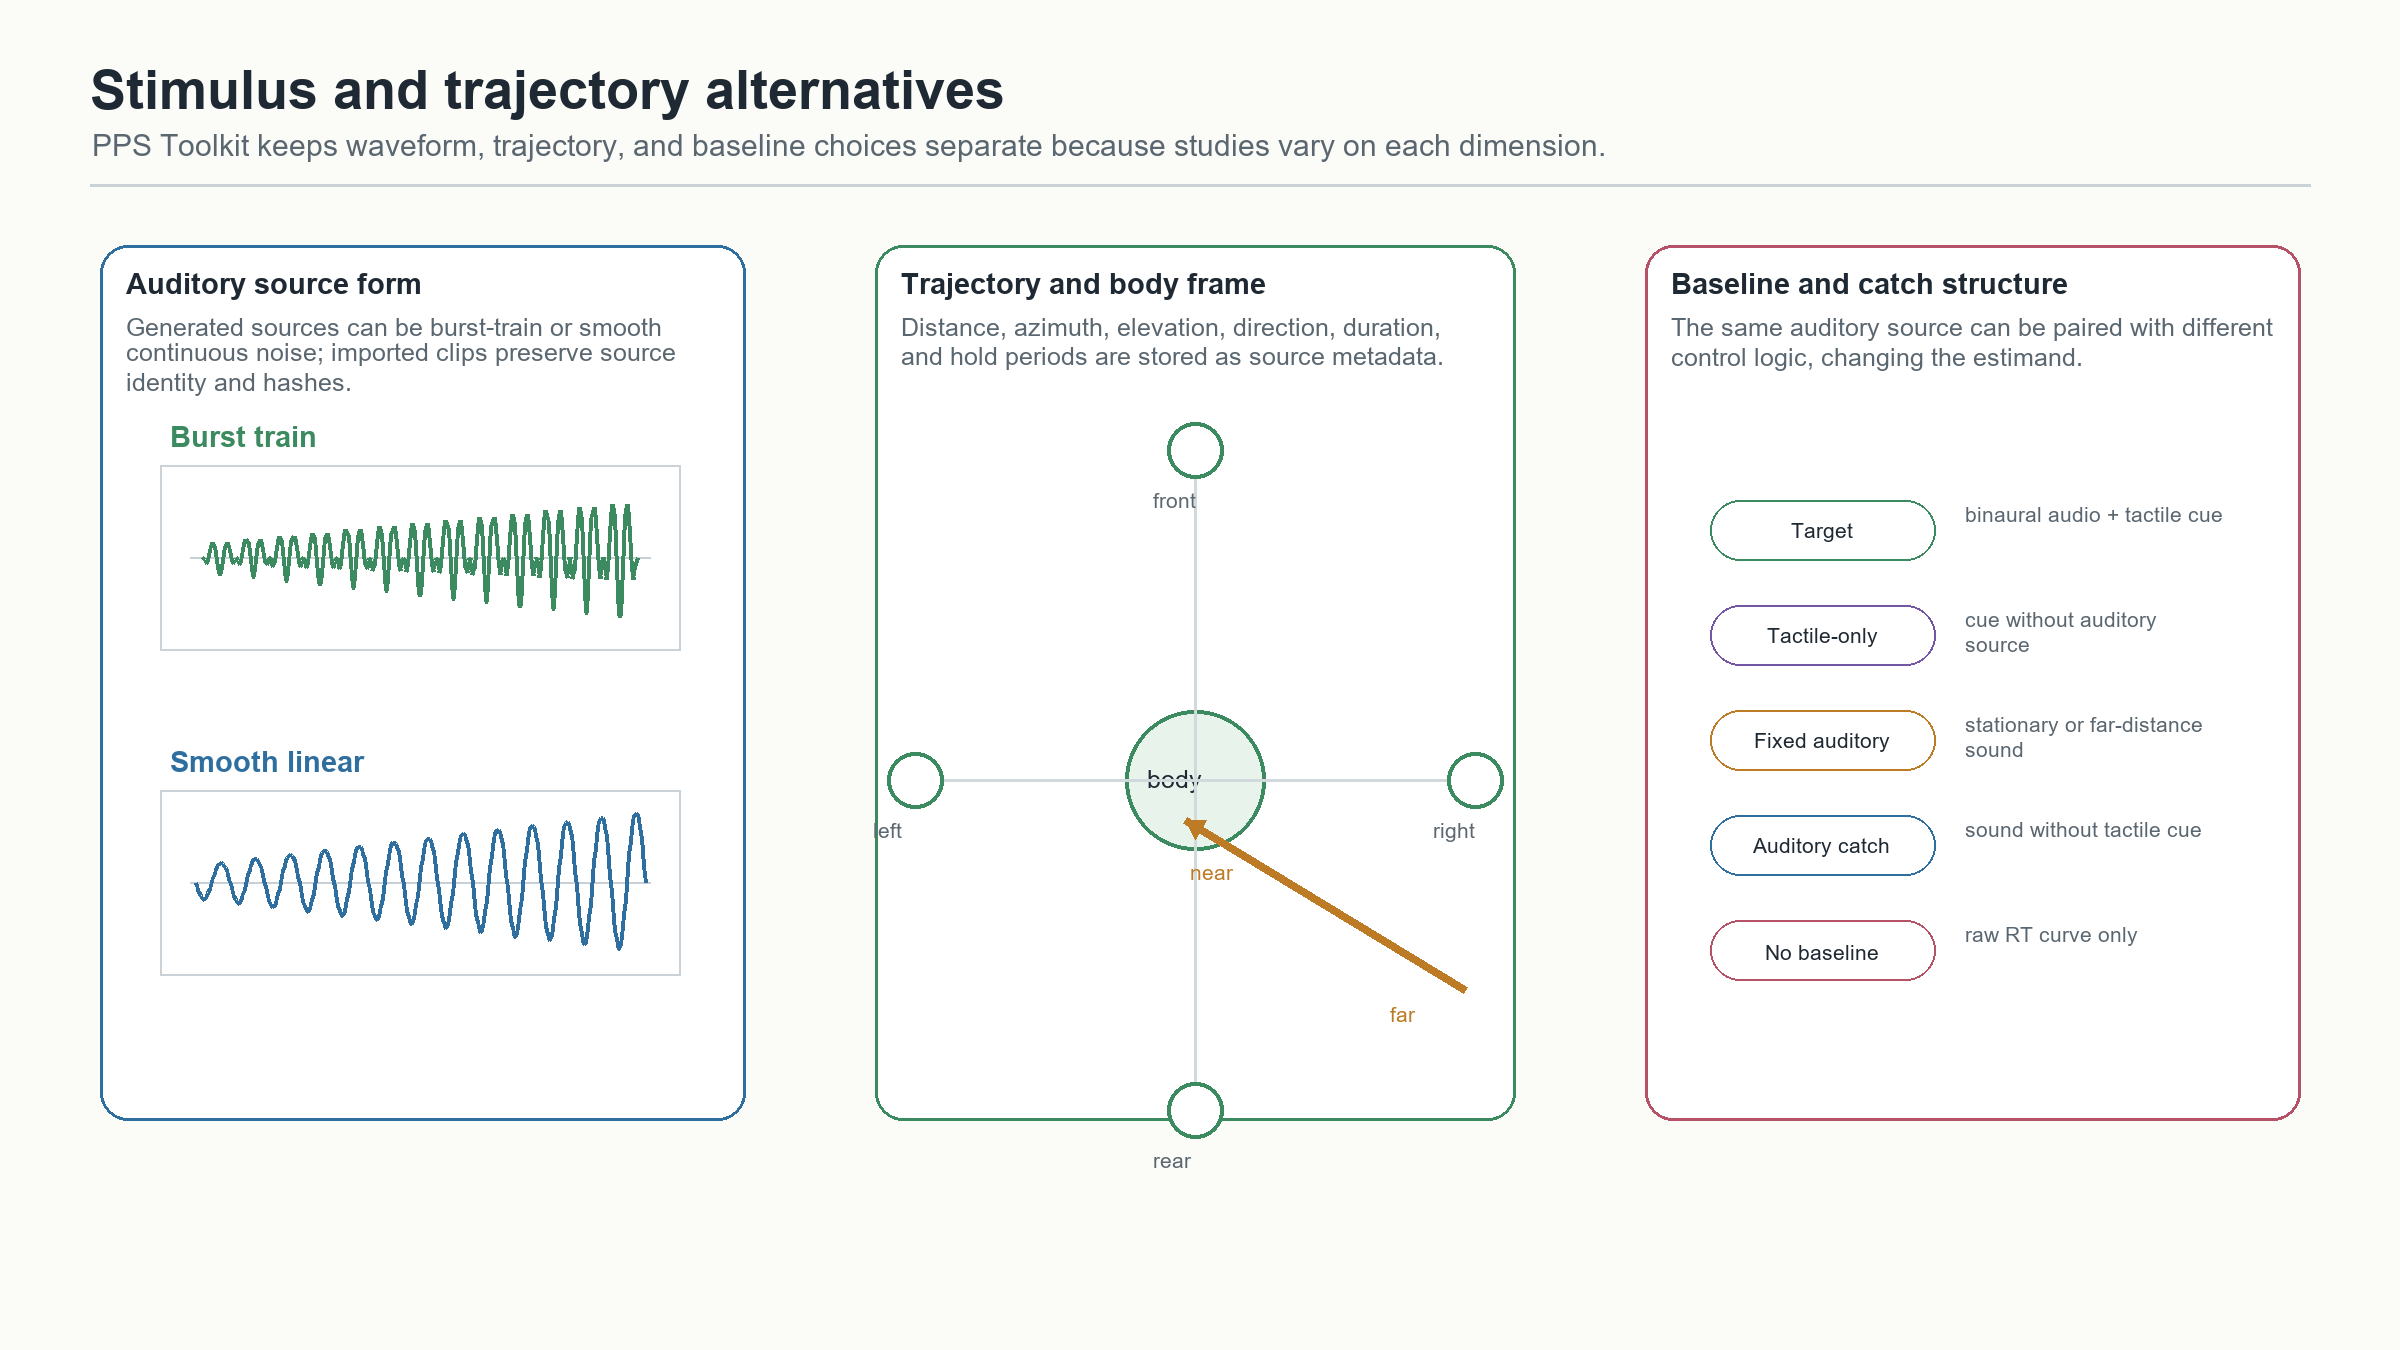
\includegraphics[width=\textwidth]{figures/figure3_stimulus_alternatives.png}
\caption{Stimulus and trajectory alternatives represented in PPS Toolkit. The figure illustrates burst-train versus smooth generated sources, body-relative trajectory metadata, and alternative target, baseline, catch, or no-baseline structures. It is a procedural schematic and does not claim perceptual equivalence to original source-paper stimuli.}
\label{fig:stimulus-alternatives}
\end{figure}

\subsection{Within-trial Sequences}

Segment 2 defines the trial families. A row can hold a breathing instruction followed by a looming source, or a jitter box, a speech clip, or a set of alternative sources sharing one temporal slot. Alternatives inside a box multiply the concrete sequence variants while they keep the row's identity fixed. A researcher can thus encode condition factors such as noise class, spatial direction, or valence without duplicating files by hand.

The sequence layer sits upstream of tactile insertion on purpose. The literature describes a PPS trial by when the tactile event falls relative to sound onset, but the sound itself may follow an instruction, a fixation, a respiratory cue, or a silent interval. Because Segment 2 stores the exact component timing, the first looming onset, the jitter duration, and the total sequence duration in its manifest, Segment 3 can place each tactile cue from that timing rather than guess it from a filename.

\subsection{Tactile and Baseline Trial Generation}

Segment 3 turns the stereo/binaural sequences into the final target, baseline, and catch assets. A target trial is a three-channel WAV file: channels 1 and 2 carry the binaural audio and channel 3 carries the tactile cue. A baseline file also carries a tactile cue, but its auditory content depends on the baseline strategy the researcher chose. A catch file is an auditory-only stereo/binaural copy with no tactile channel.

The baseline controls are deliberately more than an on/off switch, because the field's baselines are not one thing. PPS studies use tactile-only baselines, pre/post tactile controls, auditory-only catch trials, stationary or fixed-distance auditory baselines, and sometimes no correction at all.

Canzoneri-style dynamic tasks add tactile controls before and after the sound alongside auditory-only catches \citep{Canzoneri2012}. Hobeika and colleagues introduced a fixed-distance baseline to pull expectancy apart from distance-dependent audio-tactile integration \citep{Hobeika2019}. Teraoka and colleagues used a tactile-only baseline to compare front and rear spaces \citep{Teraoka2024}. Holmes and colleagues showed that response probability, control conditions, and flexible analysis choices can swing the inferred near-sound benefit \citep{Holmes2020}. Because the baseline decides what counts as facilitation, \toolkit{} treats it as a first-class design choice rather than a default.

\subsection{Repetition Pools and Block Review}

Segment 4 expands the Segment 3 assets into a CSV repetition pool. The researcher sets a global repetition count, folder-level counts, and per-WAV overrides, and the dashboard reports the total trial rows, the condition percentages, the estimated duration, and the longest folder's contribution. This addresses a recurring practical problem: a small change in baseline proportion or catch count shifts both participant burden and response probability, and a researcher needs to see that before running anyone.

Segment 5 turns the pool into block CSV files and preserves row and family order wherever the design requires it. In a Study 5-style breathing design, the inhale and exhale rows stay an alternating scaffold; the algorithm randomizes concrete trial identities within each row-family queue instead of treating all rows as exchangeable. The researcher inspects the generated blocks before accepting them. Accepting Segment 5 locks the current CSVs as final and unlocks Segment 6. This turns randomization from a hidden runtime event into a citable artifact.

\subsection{Experiment Preparation and Native Runner Handoff}

Segment 6 builds the participant-by-part schedule. The researcher sets the participant count and a one-part or two-part structure, inspects the block-order permutations, prepares the output folder, and launches the native \code{PPSExperimentRunner.exe}. The browser dashboard stays an orchestrator. The native Focus Mode runner owns everything that has to happen in real time: synchronized playback, response logging, LSL markers, optional LabRecorder capture, local audio evidence, loopback evidence, tactile threshold calibration, and missed-trial top-up.

The runner writes two layers, a minimal public-data layer and a reconstructive private session layer. The public \code{1.Data\_min} folder holds participant CSVs on a curated 17-column schema ready for publication or OSF-style sharing. The \code{2.Data\_max} mirror holds the richer reconstruction artifacts: session manifests, event logs, local marker mirrors, XDF captures, trigger dictionaries, prepared block manifests, audio evidence, top-up ledgers, calibration artifacts, and exploratory analysis outputs. The split keeps the open data usable and keeps private metadata, raw outputs, and local debugging artifacts from leaking into a public release by accident.

The manuscript source includes \code{output\_schema\_dictionary.csv}, a data dictionary for these layers. This is a methods feature, not just a repository convenience: a reader needs to know which files are meant for public reuse, which reconstruct a session, which are timing or marker evidence, and which stay private unless a release review approves them \citep{Ellis2024,Kieslich2017,Ghose2020}. Table~\ref{tab:output-schema} summarizes the boundary.

\begin{table}[t]
\caption{Output schema and archive boundary for runner-generated artifacts.}
\label{tab:output-schema}
\footnotesize
\begin{tabularx}{\textwidth}{>{\raggedright\arraybackslash}p{0.19\textwidth} >{\raggedright\arraybackslash}p{0.25\textwidth} >{\raggedright\arraybackslash}X >{\raggedright\arraybackslash}p{0.22\textwidth}}
\toprule
Layer & Main artifacts & Evidence role & Publication boundary \\
\midrule
Public response data & Participant and master CSVs in \code{1.Data\_min} & Deidentified 17-field trial summary for condition, SOA, response, hit/miss status, and RT. & Candidate public dataset after deidentification and human release review. \\
Rich reconstruction & Session trial CSVs and session files in \code{2.Data\_max} & Trial timing, response classification, top-up flags, source-trial links, manifests, hashes, and route settings. & Private/session layer unless deidentified and explicitly approved. \\
Prepared playback evidence & Block manifests, concatenated WAVs, source hashes, and loudness manifests & What the runner was prepared to play and where looming, tactile, and response-window samples were scheduled. & Share only if source assets, paths, and third-party rights are safe. \\
Event and marker evidence & Verbose event CSV/XDF, LSL marker mirror, trigger dictionary, and optional LabRecorder XDF & Software event stream, marker-push record, and external-capture reconciliation. & Validation layer; still not physical onset proof without loopback/mechanical evidence. \\
Tactile safeguards & Calibration trials/report, top-up ledger, adaptive-threshold summary, and adjustment CSV & Perceptual threshold procedure, misses, top-up decisions, and two-miss Output 3/4 nudges. & Operator and reconstruction evidence, not proof of mechanical tactile onset or habituation correction. \\
Exploratory review & Data analytics folder, timing QC, response summaries, model-fit tables, and analysis catalog & Operator-facing QC, baseline checks, low-N warnings, and exploratory model alternatives. & Not confirmatory inference unless paired with a preregistered analysis and adequate data. \\
\bottomrule
\end{tabularx}
\end{table}

\section{Design-decision Evidence Matrix}

Tables~\ref{tab:matrix-core} and \ref{tab:matrix-runner} condense the matrix; \code{evidence\_matrix.csv} holds the full editable source. The matrix is not a formal systematic review. It is a source-pointer scaffold: each row ties a literature-bearing toolkit control to the methodological variation it governs, the design rationale behind it, and the caveat a report must state.

The source package also ships \code{gui\_control\_coverage.csv}, which audits the visible dashboard at the control level and separates a scientific design decision from an execution gate, an artifact-review display, a suite boundary, or an ordinary navigation or documentation control. That separation carries the suite claim.

Camera presets, modal close buttons, folder openers, documentation tabs, and refresh controls support inspection and operation, but we do not count them as PPS design decisions unless they change provenance, materialization state, the acquisition boundary, or the runner handoff. The controls that do alter source form, trajectory, SOA, baseline, repetition, block order, participant structure, instruction behavior, or runner preparation map back to the evidence matrix and the reporting checklist, as Figure~\ref{fig:decision-map} summarizes.

\begin{table}[t]
\caption{Condensed design-decision matrix for PPS Toolkit: design and stimulus layers. The accompanying CSV contains the full row-level audit for Segment 0-6 controls and runner decisions.}
\label{tab:matrix-core}
\footnotesize
\setlength{\tabcolsep}{3pt}
\begin{tabularx}{\textwidth}{>{\raggedright\arraybackslash}p{0.16\textwidth} >{\raggedright\arraybackslash}p{0.22\textwidth} >{\raggedright\arraybackslash}X >{\raggedright\arraybackslash}p{0.17\textwidth}}
\toprule
Decision cluster & Toolkit control & Literature variation and rationale & Main caveat \\
\midrule
Dashboard mode and execution boundary & View/Edit mode; read-only bundled profiles; hosted/static preview; local companion/native runner & Experiment builders improve reuse, but timing-sensitive behavioral software must keep runnable assets and validation evidence inspectable \citep{AnwylIrvine2018,Peirce2019,Bridges2020,Ellis2024}. & A hosted preview is not acquisition or timing evidence. \\
Artifact materialization gates & Apply, Bake, Accept Blocks, Prepare Output Folder, and Start Experiment Runner actions & Runnable behavioral software needs self-documenting task logic, reusable operational assets, and validation before data interpretation \citep{AnwylIrvine2018,Akam2022,DeLeeuw2022,Ellis2024}. & Completed gates show artifact consistency, not hardware timing or theoretical correctness. \\
Auditory source form & Burst-train or smooth generated sources; imported custom sounds & PPS studies use continuous noise, burst trains, rough sounds, and affective/ecological sounds \citep{Canzoneri2012,Farne2002,Hug2019,Taffou2021,Roussel2025}. & Source mode is not a control condition unless it is explicitly crossed and analyzed. \\
Loudness and gain law & Segment 1 loudness contract; start/end level policy; instruction offset; peak ceiling & Auditory distance judgments depend on level, source spectrum, reverberation, and normalization choices \citep{Zahorik2002,Kolarik2015,Spagnol2017,Arend2021Level}. & Estimated SPL is not a substitute for measured acoustic calibration. \\
Trajectory and spatial frame & Distance, azimuth, elevation, direction, duration, speed & Front/rear/left/right, walking, and 3D tasks show that PPS is body-relative and direction-sensitive \citep{Matsuda2021,Noel2015,Teraoka2024,Amiel2025}. & Binaural trajectories approximate apparatus geometry; unsupported social or VR context remains metadata. \\
Spatial rendering & SOFA/FABIAN reference path and 3DTI-compatible manifests & Near-field HRTFs, renderer interpolation, and open binaural engines matter for peribody distances \citep{Salvador2018,CuevasRodriguez2019,Hoene2017}. & Generic rendering is not individualized localization evidence. \\
Trial sequence design & Row/family builder, ordered audio boxes, alternatives, jitter & PPS timing often combines task instructions, sound onset, SOA, and response windows; expectancy is a known confound \citep{Hobeika2019,Holmes2020}. & Some papers require ITI or apparatus details not yet exposed as first-class controls. \\
Baseline and control logic & Tactile-only, stationary/fixed-distance, min/max anchor, full-SOA, catch files & Baseline practice differs across Canzoneri-style controls, Hobeika fixed-distance correction, Teraoka tactile-only baselines, and critique of missing controls \citep{Canzoneri2012,Hobeika2019,Teraoka2024,Holmes2020}. & No baseline is universally correct; manuscripts must justify the chosen correction. \\
\bottomrule
\end{tabularx}
\end{table}

\begin{table}[t]
\caption{Condensed design-decision matrix for PPS Toolkit: runner, randomization, and analysis layers.}
\label{tab:matrix-runner}
\footnotesize
\setlength{\tabcolsep}{3pt}
\begin{tabularx}{\textwidth}{>{\raggedright\arraybackslash}p{0.16\textwidth} >{\raggedright\arraybackslash}p{0.22\textwidth} >{\raggedright\arraybackslash}X >{\raggedright\arraybackslash}p{0.17\textwidth}}
\toprule
Decision cluster & Toolkit control & Literature variation and rationale & Main caveat \\
\midrule
Tactile calibration and misses & Pre-run threshold assay; run-local adaptive nudge after repeated misses & Vibrotactile thresholds vary with method, reliability, and adaptation \citep{Merchel2020,Mikkelsen2020,Morioka2002,Goble1993,Pate2024}. & Pilot miss-rate observations are anecdotal until tied to traceable artifacts. \\
Randomization and blocks & Repetition pools, seeded distribution, block acceptance, participant permutations & Reproducible experiment-builder workflows benefit from saved schedules and auditable randomization \citep{AnwylIrvine2018,Peirce2019,Ellis2024}. & Randomization artifacts do not replace preregistration or power analysis. \\
Response rule and classification & Participant response target; tactile-onset response window; catch and top-up labels & RT-based PPS inference is sensitive to response probability, catch errors, and response-device timing \citep{Holmes2020,Canzoneri2012,Roussel2025,Bridges2020}. & Classification rules audit responses; they do not validate tactile perception or a PPS effect. \\
Analysis choices & Raw RT curves, baseline-corrected facilitation, sigmoid, log-decay, linear fits & Canonical sigmoid boundaries and logarithmic/linear distance arguments coexist with small-effect and control-condition critiques \citep{Canzoneri2012,Hobeika2019,Holmes2020}. & Instant analysis is exploratory operator feedback, not confirmatory inference. \\
\bottomrule
\end{tabularx}
\end{table}

\subsection{Profile and Provenance Decisions}

Segment 0 is more than a convenience selector. Published PPS paradigms differ in small but consequential ways: body part, sound direction, baseline type, catch-trial policy, response modality, and the criterion used to fit the boundary. The profile registry surfaces that translation before anyone runs the experiment.

A bundled profile can be a verified implementation of the fields the toolkit represents, a partial scaffold for a paper with missing apparatus details, or a custom project with local-only assets. Marking which one it is heads off a common failure of methods reuse, in which a laboratory inherits a task label such as ``Canzoneri-style dynamic sounds'' without inheriting the assumptions that made the task interpretable.

The same logic governs project naming, citation export, and profile snapshots. A PPS design is not a set of sound files. It is a relationship among source identity, trajectory, SOA, tactile cue, baseline rows, block order, and analysis plan. Segment 0 stores that relationship as a reusable project instead of a one-off folder. For a BRM readership the registry is part of the method, because it is what lets another lab inspect, copy, and criticize the same design.

\subsection{Auditory Source, Trajectory, and Rendering Decisions}

Segment 1 exposes source form because the field has never converged on one auditory stimulus. Continuous or smoothly enveloped looming noise carries a stable motion cue; burst trains supply salient repeated onsets that aid detection and match recent DynaSpace and mobile implementations. Rough, affective, speech, animal, and ecological sounds add semantic or defensive value on top of distance information \citep{Taffou2021,Ferri2015,Bahadori2021,Tonelli2019}.

The source-mode toggle is therefore not cosmetic. It forces the researcher to decide whether the approaching event is a smooth motion signal, a punctate warning-like train, or a locally imported stimulus with its own provenance, because that decision shapes how participants respond.

The loudness contract belongs to the same Segment 1 decision layer. A dynamic sound can approach by shifting binaural and spatial cues, by rising in level, by changing the direct-to-reverberant ratio, or by combining these. Listeners weight those cues flexibly, so a nominal distance manipulation quietly becomes a loudness manipulation whenever the gain law goes undocumented \citep{Zahorik2002,Kolarik2015}.

The toolkit therefore records level targets and renderer gain behavior as methods metadata. Doing so does not promote an estimated hardware specification to a measured SPL. It exposes the measurement boundary, so a submitted study can swap the estimate for coupler/HATS or other calibrated acoustic evidence.

Trajectory controls are methodological for the same reason. A dynamic PPS task reads SOA through the sound's estimated position at tactile onset, and that estimate depends on start distance, end distance, speed, approach or recede direction, azimuth, elevation, and the coordinate frame fixed to the body. Front, rear, left, right, trunk-centered, hand-centered, and full-body designs are not interchangeable \citep{Matsuda2021,Teraoka2024,Amiel2025,Serino2015,Noel2015}. The toolkit therefore stores trajectory samples and body-relative labels rather than assume a list of SOAs will do.

The toolkit treats spatial rendering metadata as provenance, not magic. A 3D Tune-In-style renderer gives an open, documented binaural path with HRTF convolution, ITD handling, near-field processing, and moving-source safeguards \citep{CuevasRodriguez2019}. SOFA-style HRTF resources keep the renderer inputs portable, and near-distance HRTF work matters directly here because many PPS distances fall below one meter \citep{Salvador2018}.

Virtual near-field distance nonetheless stays hard. Real and rendered nearby sources can split in distance judgments, distance-variation filtering helps some near-lateral judgments without removing distance uncertainty, and near-field cues do not always improve plausibility under non-individualized rendering \citep{Parseihian2014,Kan2009,Spagnol2017,Arend2021}. The toolkit therefore records the HRTF and renderer choices as reportable provenance, not as proof that participants perceived the intended space.

\subsection{Within-trial Sequence, SOA, Baseline, and Catch Decisions}

Segment 2 exists because a PPS trial is usually more than a sound plus a tactile pulse. It may carry breathing instructions, a fixation or silence, a jitter interval, a local instruction clip, or alternatives that define condition factors. Hide those temporal components until WAV synthesis and later analysis can no longer tell whether a tactile SOA was measured from file onset, instruction offset, looming onset, or some other anchor. The row-and-box model keeps the trial's temporal grammar inspectable before any tactile event goes in.

Segment 3 is where the core inferential choices of a PPS task land. The SOA values set the intended contact points between tactile detection and sound distance. The baseline choice sets what counts as facilitation.

A tactile-only baseline asks how fast the participant responds with no auditory probe at all. A stationary or fixed-distance baseline asks how much of the response reflects expectancy or the mere presence of audio rather than approach. A pre/post tactile control samples tactile responses outside the moving-sound window. Catch trials ask whether the participant responds when no tactile event occurs. These are different controls, not settings of one checkbox \citep{Canzoneri2012,Hobeika2019,Teraoka2024,Holmes2020}.

The toolkit keeps the variants explicit because the baseline can change the scientific reading of the same data. Holmes and colleagues make the constructive point: leave response probability, trial counts, expectancy, and control conditions unreported, and a near-versus-far benefit turns ambiguous \citep{Holmes2020}. The toolkit cannot decide which baseline is theoretically right for every study, but it can force the baseline to be named, materialized, hashed, scheduled, and carried through into the analysis artifacts.

\subsection{Repetition, Randomization, Participant Structure, and Runner Decisions}

Segments 4 and 5 treat trial counts and randomization as methods artifacts. PPS studies differ in repetitions per SOA, catch proportion, block factors, and direction balancing, and those decisions drive response probability, fatigue, statistical precision, and whether a model can be fit at all. The repetition pool and block preview put the actual trial composition in front of the researcher before any participant arrives.

Segment 5 also protects within-trial family structure. Some protocols demand a meaningful row order, such as alternating inhale and exhale families or a direction-specific sequence; others allow freer randomization. Constrained sequence generation has a long history in behavioral methods, because naive randomization produces clusters while ad hoc constraints introduce their own sequential structure \citep{Jadoul2023,French2009}.

The toolkit's seeded, inspectable block generation therefore makes a concrete schedule an object the researcher reviews, not an invisible runtime side effect. The researcher can accept the schedule, regenerate it, or download it for reporting. This follows the broader behavioral-software lesson that experiment logic should be testable and reconstructable, not merely executable \citep{DeLeeuw2022,Ellis2024}.

Segment 6 draws the line between study design and runtime acquisition. The browser prepares the participant order, the one-part or two-part structure, the profile snapshots, and the output folders; the native runner owns timing-sensitive playback, responses, LSL markers, LabRecorder capture, and the local evidence files. The line matters because timing validation depends on the hardware and configuration. Broad timing comparisons show that platforms diverge across operating systems, browsers, audio paths, and response devices \citep{Bridges2020}. The toolkit therefore counts the local validation outputs as part of the methods package, not as optional troubleshooting.

\subsection{Tactile Calibration, Top-up, and Analysis Decisions}

The tactile-calibration controls expose a real tension in running the task. Individual calibration is worth doing because vibrotactile thresholds vary across participants and measurement procedures \citep{Merchel2020,Mikkelsen2020,Morioka2002,Pate2024}. Yet a calibrated near-threshold stimulus can raise misses over a long task, and vibrotactile adaptation can lift detection thresholds over time, with recovery and peripheral time courses that depend on stimulus history and receptor class \citep{Goble1993,Hollins1990,Leung2005}. The runner's two-miss output nudge is a narrow operational answer to that risk. The runner logs it as evidence, caps it, and never writes it back as a new calibration estimate.

Missed-trial top-up is likewise a safeguard, not a statistical cure. It restores a participant's exposure to the planned tactile trials and makes the missingness visible to the operator. It cannot unmake the original miss, and it must not fold silently into the primary RT estimate. The analysis layer therefore shows hits, misses, catch false alarms, top-up rows, and low-N warnings before it shows a single model fit.

The instant-analysis model buttons are plural on purpose. A sigmoid summarizes PPS as a transition between far and near space, while a logarithmic-decay or linear summary fits a graded reading of distance-dependent facilitation \citep{Canzoneri2012,Hobeika2019}. The toolkit lets the researcher compare these alternatives quickly, but labels them exploratory unless the study brings a preregistered model, adequate cell counts, and a declared baseline correction.

\section{Reporting Checklist}

The evidence matrix supports reporting, not just development. Table~\ref{tab:reporting} gives a minimum checklist for a manuscript, preregistration, or shared profile built with \toolkit{}. The checklist separates what the software documents directly from what still needs laboratory validation or participant data.

\begin{table}[t]
\caption{Minimum reporting checklist for PPS Toolkit experiments.}
\label{tab:reporting}
\footnotesize
\begin{tabularx}{\textwidth}{>{\raggedright\arraybackslash}p{0.20\textwidth} >{\raggedright\arraybackslash}X >{\raggedright\arraybackslash}p{0.26\textwidth}}
\toprule
Topic & Report from toolkit artifacts & Boundary to state \\
\midrule
Profile and provenance & Profile id, project id, profile citation, verification status, design manifest hash, and local asset exceptions. & A profile is a represented implementation, not proof of exact original-apparatus equivalence. \\
Dashboard state and execution boundary & View/Edit state, bundled or custom profile status, hosted/static versus local-companion mode, and whether acquisition was run in the native runner. & Read-only preview, editable design work, and timing-sensitive acquisition are different evidence states. \\
Materialization gates & Applied profile/project id, each Segment 1-6 bake or prepare action, consumed upstream hash, written artifact manifest, accepted block state, stale-state warnings, and runner handoff package id. & A completed GUI gate documents artifact provenance; it does not prove participant timing, acoustic output, tactile onset, or scientific validity. \\
Auditory source and trajectory & Source mode, imported or generated asset hashes, start/end distance, azimuth, elevation, duration, speed, looming/receding label, and body-relative frame. & Source class and trajectory are manipulations; do not relabel them as controls unless crossed in the design. \\
Spatial rendering & SOFA/HRTF resource, renderer path or engine, trajectory sample table, channel layout, and renderer QC files. & Renderer provenance does not establish individualized localization, externalization, or perceived distance. \\
Auditory level & Loudness policy, start/end SPL targets, instruction offset, peak ceiling, gain-law mode, hardware estimate or measured calibration file. & Estimated SPL and measured participant-ear SPL are different evidence layers. \\
Trial sequence and SOA & Sequence rows, audio boxes, jitter durations, looming onset anchor, tactile SOAs, response windows, and catch rules. & SOA interpretation depends on the temporal anchor used for tactile insertion. \\
Baseline and repetition pool & Baseline strategy, baseline SOAs, stationary/fixed-distance source files, catch proportion, repetition counts, and condition totals. & Baseline correction changes the estimand; raw and corrected curves remain distinguishable. \\
Randomization and participant structure & Random seed, accepted block CSVs, family-order constraints, participant block-order manifest, and one-part or two-part schedule. & Constrained randomization should be justified and inspectable; it does not replace counterbalancing. \\
Runner and validation evidence & Output levels, tactile threshold file, adaptive-threshold log, top-up ledger, event logs, LSL/XDF files, audio evidence, and loopback report when available. & Software, digital audio, electrical loopback, mechanical tactile output, and perception are separate evidence tiers. \\
Response classification & Response device, tactile-onset anchor, valid RT window, anticipation/late-click rule, catch false-alarm rule, miss/top-up policy, and selected click identifiers. & RT curves are interpretable only after response probability, catch performance, and exclusion rules are stated. \\
Analysis & Response integrity summary, baseline method, included trials, exclusion rules, model families, AICc table, low-N warnings, and exploratory labels. & Instant analysis is review support unless the model and exclusions were prespecified. \\
\bottomrule
\end{tabularx}
\end{table}

\section{Design, Run, and Recreation Pathway}

A BRM methods paper should leave the reader with an executable path, not only a conceptual argument. \toolkit{} offers three entry points into that path. The suite framing matters here: the contribution is not just a dashboard for designing stimuli but a design-run-recreation system that turns a PPS method into an executable, inspectable experiment. It meets the expectation behavioral software papers share, that a graphical tool should lower the programming barrier while it keeps timing, task logic, and open-science materials inspectable \citep{AnwylIrvine2018,Peirce2019,Akam2022}.

\begin{table}[t]
\caption{Three practical entry points through PPS Toolkit.}
\label{tab:entrypoints}
\footnotesize
\begin{tabularx}{\textwidth}{>{\raggedright\arraybackslash}p{0.18\textwidth} >{\raggedright\arraybackslash}p{0.22\textwidth} >{\raggedright\arraybackslash}X >{\raggedright\arraybackslash}p{0.22\textwidth}}
\toprule
Entry point & Starting object & Primary toolkit actions & Evidence boundary \\
\midrule
New-study design & Custom project & Define auditory sources and trajectories, assemble sequence rows, choose baseline/catch logic, set repetitions, and accept block CSVs. & Produces a design archive; it does not prove participant effects. \\
Published-profile recreation & Bundled profile & Inspect citation, verification status, represented fields, and caveats; copy into an editable project when adapting the profile. & A profile is an implementation scaffold unless original methods and assets are fully verified. \\
Native acquisition & Accepted Segment 6 package & Launch Focus Mode for setup, output checks, tactile calibration, synchronized playback, response logging, LSL/LabRecorder/event mirrors, optional loopback, top-up, and analysis artifacts. & Runner evidence is separate from hardware timing, tactile mechanics, and participant perception. \\
\bottomrule
\end{tabularx}
\end{table}

A researcher should archive the resulting package in layers rather than as one undifferentiated experiment folder. Table~\ref{tab:archive-layers} names those layers and the claim each one can support.

\begin{table}[t]
\caption{Recommended archive layers for PPS Toolkit studies.}
\label{tab:archive-layers}
\footnotesize
\begin{tabularx}{\textwidth}{>{\raggedright\arraybackslash}p{0.20\textwidth} >{\raggedright\arraybackslash}X >{\raggedright\arraybackslash}p{0.25\textwidth}}
\toprule
Archive layer & Include & Claim supported \\
\midrule
Design archive & Profile snapshot, manifest chain, source hashes, accepted block CSVs, and evidence-matrix rows for unusual choices. & The experiment was specified and can be inspected or rebuilt. \\
Profile-recreation archive & Source-paper pointer, represented parameters, missing or approximated fields, profile status, and local substitutions. & A published paradigm was translated into an auditable scaffold. \\
Validation archive & Software run, operating-system and hardware route, event logs, digital audio evidence, optional LSL/XDF captures, and optional electrical loopback reports. & The prepared package executed on a stated route with stated evidence tiers. \\
Participant archive & Deidentified analysis-ready rows plus declared response-window, exclusion, baseline, and model-fitting rules. & Participant data can be interpreted without exposing private acquisition artifacts. \\
\bottomrule
\end{tabularx}
\end{table}

Keeping these layers apart is not clerical overhead. Computational reproducibility studies show that a research asset can be public yet still resist execution, and that a simulation or validation tool can expose an experiment error before anyone interprets participant data \citep{Ellis2024,DeLeeuw2022}. The practical suite claim is therefore conditional: another lab can design a new task, recreate a reported paradigm as an auditable profile, and run the accepted design through the native evidence pipeline, but it must still validate any new hardware route, tactile actuator, HRTF choice, original-stimulus substitution, or participant population locally.

\section{Technical Method}

\subsection{Auditory Level and Loudness Policy}

\toolkit{} stores auditory level as a design contract, not a hidden gain slider. A Segment 1 manifest records the start and endpoint SPL targets, the instruction-clip offset, the peak ceiling, the distance-gain mode, the calibration-window definition, and whether each value came from an estimated hardware profile or a measured acoustic one. The default Study 5-oriented policy estimates the Komplete Audio 6 MK2 and Sennheiser HD 560S playback chain for convenience, and we treat that estimate as a placeholder until direct participant-ear acoustic measurement replaces it.

This level policy is methodological because listeners weight distance cues. Sound level, reverberation, direct-to-reverberant ratio, spectrum, source type, and normalization all move perceived distance \citep{Zahorik2002,Kolarik2015}. In near-field virtual rendering, intensity can dominate the subtler cues, and level normalization can strip useful distance information or leave a misleading residual cue \citep{Spagnol2017,Arend2021Level}. The toolkit therefore reports the gain law and loudness policy next to the trajectory and HRTF provenance. A participant study must replace any estimated SPL policy with measured acoustic calibration before it claims a participant-ear SPL, and it must keep digital output level, electrical loopback, and acoustic participant-ear SPL as separate evidence layers.

\subsection{Spatial Audio and HRTF Resources}

\toolkit{} renders the auditory sources as binaural channels from the source trajectories and a renderer manifest, and records the SOFA/HRTF resource, the renderer engine, the trajectory samples, the channel layout, and the file hashes. When no native 3D Tune-In-compatible executable is present, the default public reference path runs the FABIAN/TU Berlin HRIR resource through a Python SOFA reference renderer. The native path follows 3D Tune-In-style spatialization, with HRTF convolution, ITD handling, distance attenuation, and near-field processing \citep{CuevasRodriguez2019}. SOFA matters because it is the standard container for spatial acoustic data \citep{AES69}, and near-distance HRTF resources matter because a PPS experiment often simulates sources within one meter of the body \citep{Salvador2018}.

We report this layer conservatively. A renderer delivers consistent binaural cues and reproducible files, but it does not prove that every participant perceived the same distance, externalization, or front/back position. Near-field rendering studies show why the distinction matters: intensity, binaural filtering, distance-dependent HRTFs, head movement, and visual or proprioceptive context all shift how a listener judges a nearby virtual source \citep{Parseihian2014,Kan2009,Spagnol2017,Arend2021}. The toolkit therefore treats HRTF metadata as stimulus provenance. Individualized HRTFs, a perceptual localization check, or externalization ratings would add validation layers; the renderer does not supply them by assumption.

\subsection{Audio-tactile Output and Event Evidence}

The runner prepares the participant blocks as multichannel WAV assets and plays them through the lab audio interface. Channels 1 and 2 carry binaural headphone output. Channel 3 carries the tactile cue, and on a canonical four-channel route output 4 mirrors the tactile channel as an analog duplicate proxy. The runner anchors every planned event time to an audio sample position and mirrors it through local event logs, rich LSL markers, numeric trigger codes, and optional LabRecorder XDF capture.

The toolkit keeps four evidence tiers apart. Software-schedule evidence records the planned trial starts, looming onsets, tactile onsets, response windows, and sample positions. Digital audio evidence records the mixed output buffers the runner tried to play. Electrical loopback evidence records an analog return path, such as the output-4 tactile mirror patched back into an input. Tactile perceptual evidence comes from the participant's calibration and responses.

The tiers answer different questions. Electrical loopback checks an audio-interface route; it does not measure Woojer mechanical vibration onset or tactile sensation. Local audio evidence proves which samples were mixed; it does not prove what the participant felt.

Figure~\ref{fig:evidence-tiers} lays this chain out. The point for reporting is plain: HRTF provenance, event timing, audio-buffer evidence, loopback evidence, and tactile perceptual evidence must not collapse into one validation label.

\begin{figure}[t]
\centering
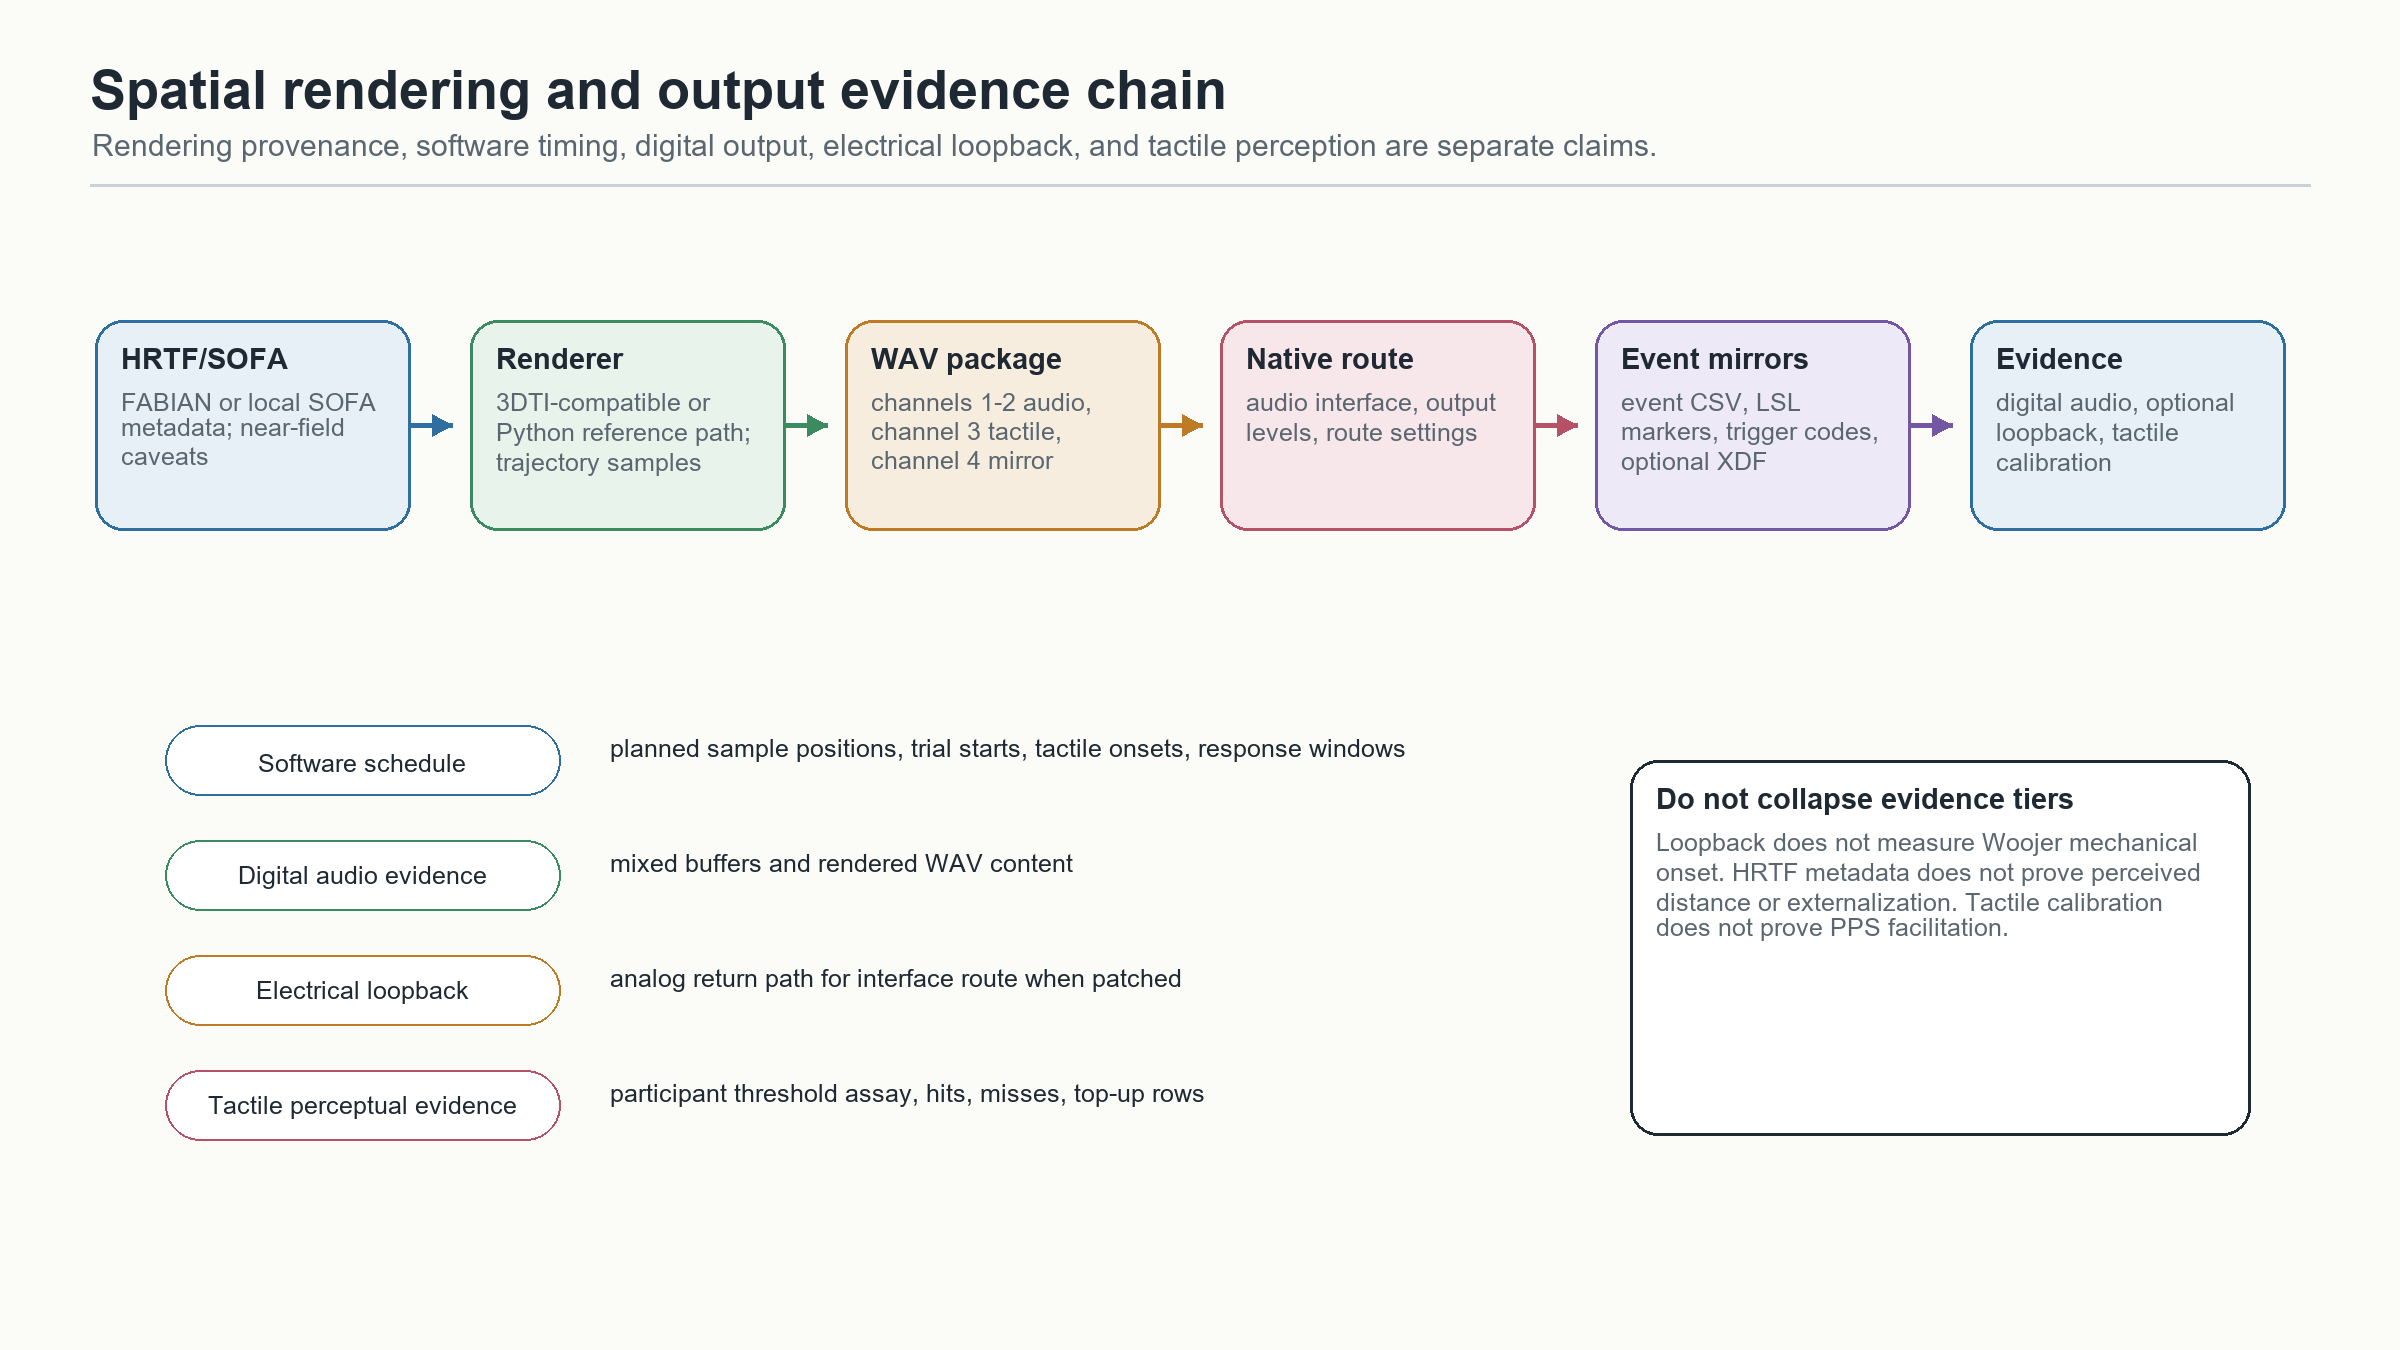
\includegraphics[width=\textwidth]{figures/figure4_evidence_tiers.png}
\caption{Spatial-rendering and output-evidence chain. The schematic separates HRTF/SOFA provenance, rendering, multichannel package construction, native route settings, event mirrors, digital audio evidence, electrical loopback, and tactile perceptual evidence. These tiers support different claims and should be reported separately.}
\label{fig:evidence-tiers}
\end{figure}

Response classification is part of the runtime method, not an afterthought. The Focus Mode runner assigns a participant click to a tactile onset through a tactile-onset-anchored valid window of 100 to 1300 ms. It keeps earlier and later clicks in the event record but does not credit them as valid tactile responses, and the next trial start does not cut short a still-open tactile deadline. The runner classifies catch trials separately as correct no-responses or false alarms, and it can mark a missed standard trial for optional top-up while it preserves the selected click identifiers.

These rules make response probability, anticipations, late responses, and rescue trials visible before anyone interprets an RT curve. That visibility matters because response probability and trial composition can manufacture an apparent near-far benefit \citep{Holmes2020}. The rules are operational defaults; a confirmatory study still has to preregister or justify them.

\subsection{Tactile Threshold Calibration}

Focus Mode runs a participant-specific tactile detection-threshold assay named \code{two\_down\_one\_up\_detection\_threshold.v2}. The assay drives a transformed adaptive staircase over a fine Output 3/4 range from 0.01\% to 0.5\%, includes catch trials, and demands a confirmation phase of consecutive tactile hits and clean catch responses before it saves a participant preset.

Tactile psychophysics motivates the procedure: vibrotactile thresholds vary across participants and methods, a detection threshold can be reliable yet method-dependent, and adaptation can lift the threshold during sustained stimulation \citep{Merchel2020,Mikkelsen2020,Morioka2002,Goble1993,Hollins1990,Leung2005}.

The runner also applies a narrow run-local safeguard. After every two tactile misses, top-up misses included, it raises the live Output 3/4 level by 0.01 percentage points up to the 0.5\% cap. It logs \code{tactile\_threshold\_adapted} events and writes \code{adaptive\_tactile\_threshold\_summary.json} and \code{adaptive\_tactile\_threshold\_adjustments.csv} to the runner-log folder.

Figure~\ref{fig:tactile-safeguards} summarizes the tactile-safeguard pathway. It is included because threshold calibration, missed trials, adaptive output changes, and top-up can otherwise disappear from the methods narrative even though they affect response probability.

\begin{figure}[t]
\centering
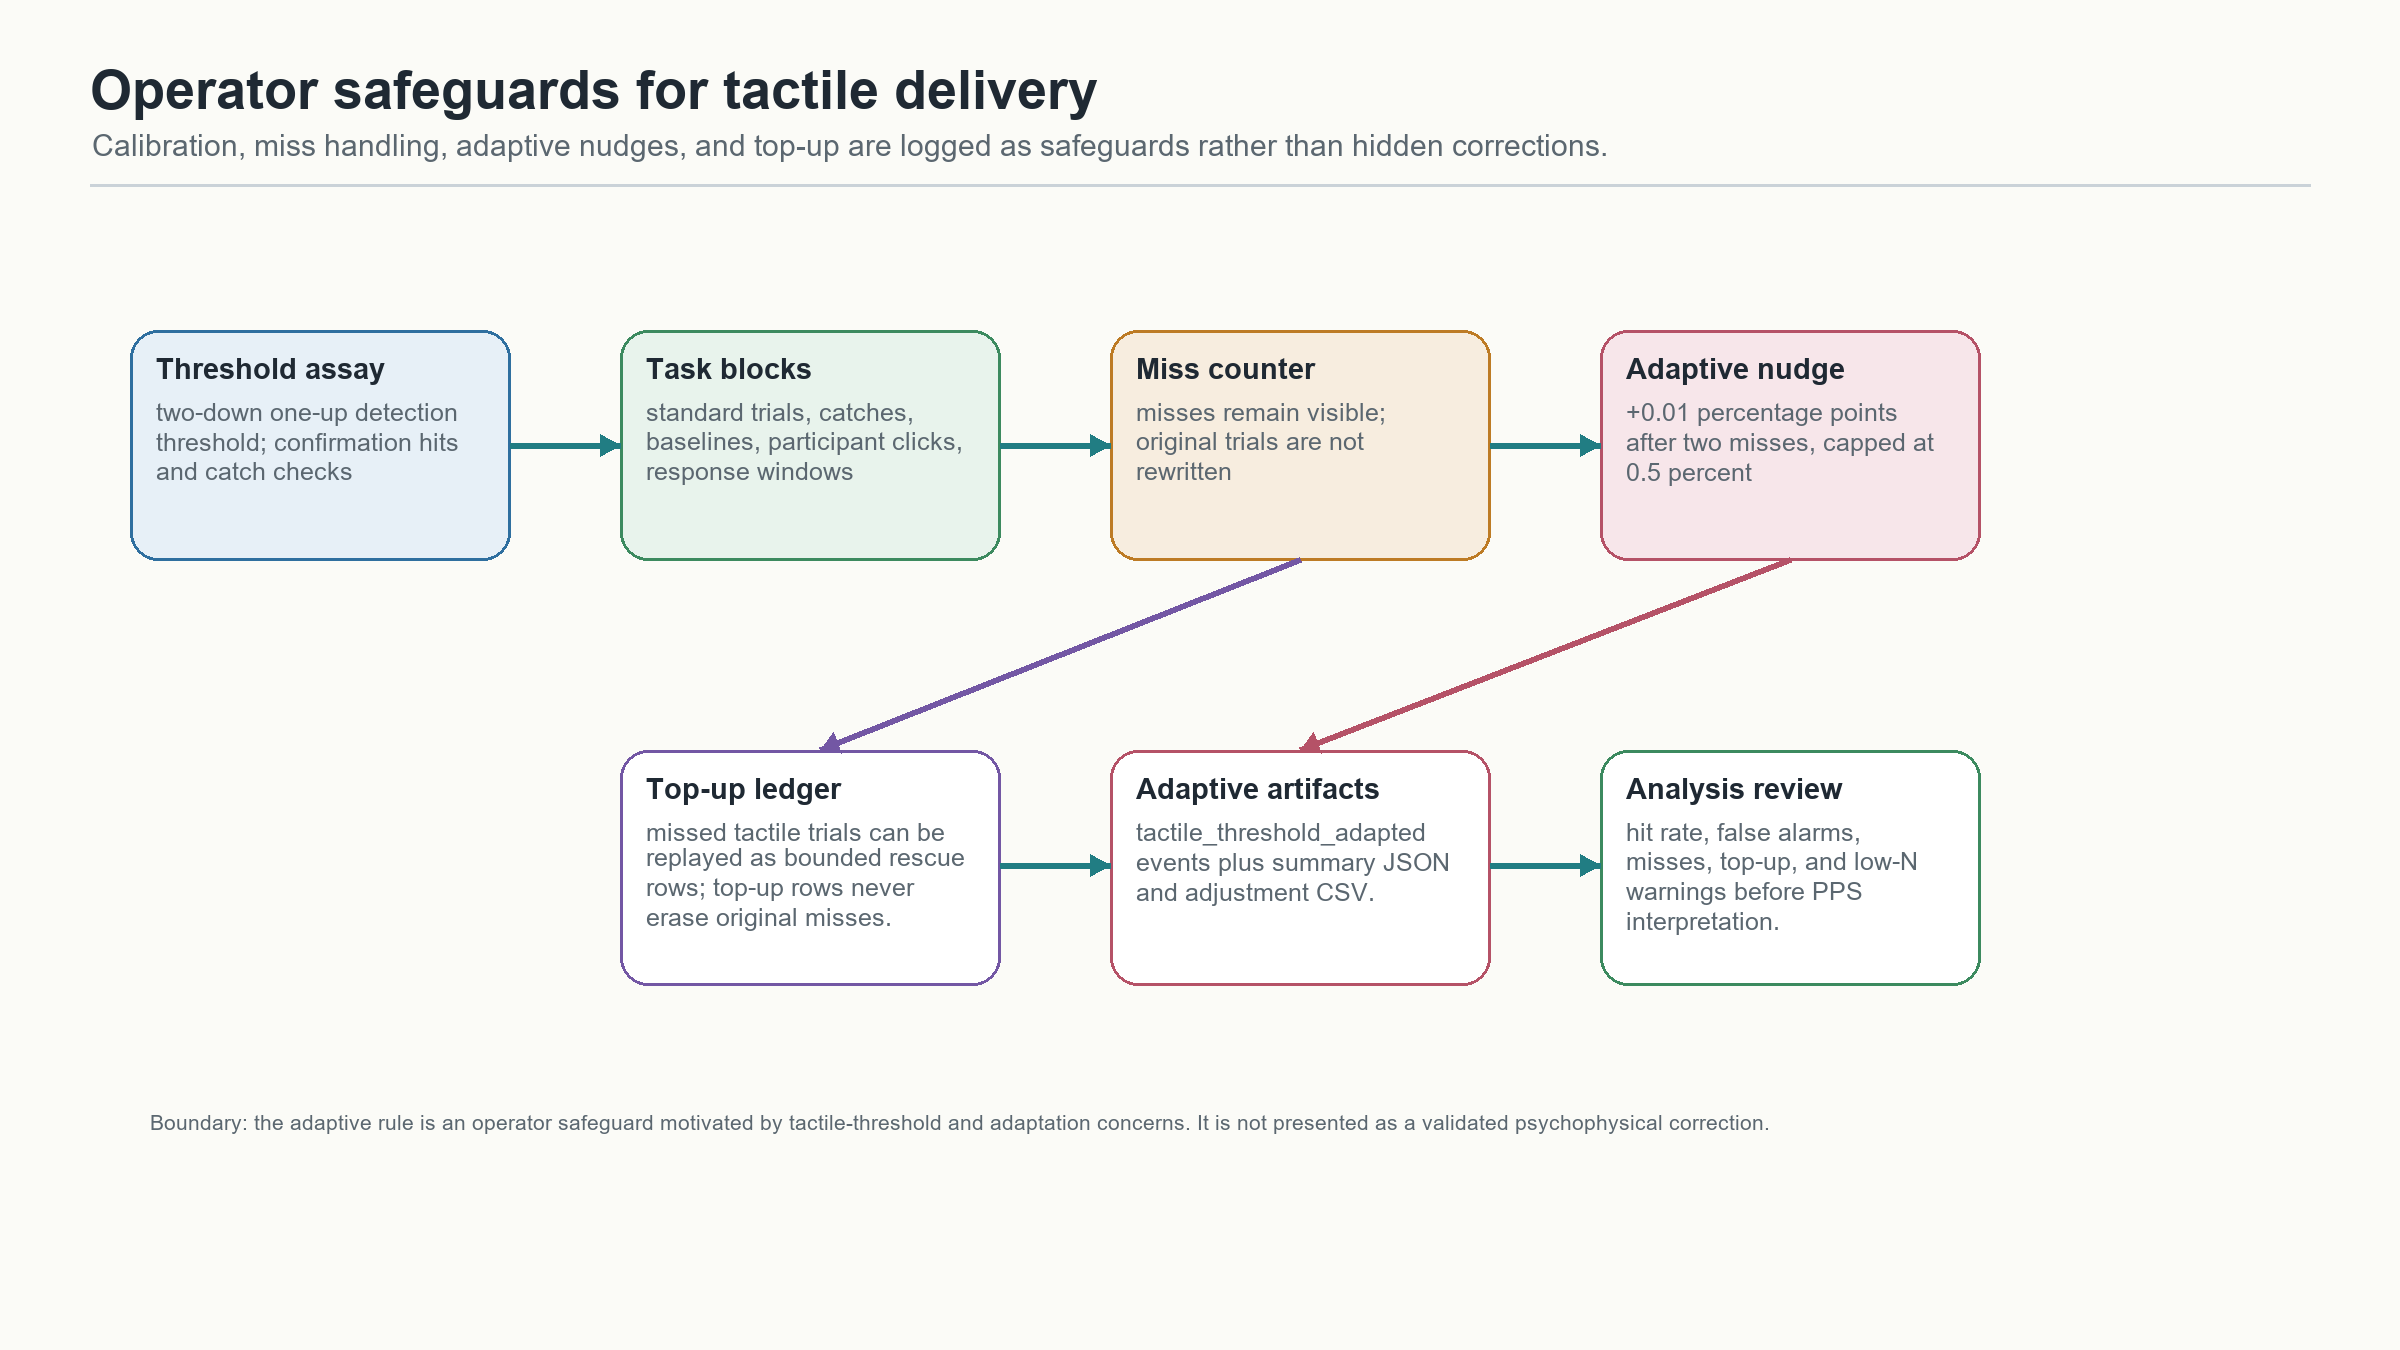
\includegraphics[width=\textwidth]{figures/figure5_tactile_safeguards.png}
\caption{Operator safeguards for tactile delivery. The figure shows the threshold assay, task blocks, miss counter, adaptive nudge, top-up ledger, adaptive-threshold artifacts, and analysis review as logged procedural steps. The adaptive nudge is presented as an operator safeguard, not as validated correction for tactile habituation or changing sensitivity.}
\label{fig:tactile-safeguards}
\end{figure}

This rule is an operator safeguard, not a validated correction for tactile habituation. We retain the observation that hit rates fell during a long calibrated task as anecdotal motivation only, until a traceable dataset and analysis artifact back it.

\subsection{Analysis Outputs}

The post-run analysis layer is exploratory by design. It shows response quality first: tactile hits, tactile misses, catch correct no-responses, catch false alarms, and top-up rows when present. It then shows basic assumption checks and model fits. A baseline-corrected curve uses one tactile-only or baseline mean per displayed condition scope, pooled across baseline SOAs, and stores \code{baseline\_correction\_method=condition\_mean\_pooled\_soa}, \code{baseline\_n}, and \code{baseline\_source\_soas\_ms}. When no usable baseline exists, the plots and fits fall back to raw mean reaction time.

The model choices span sigmoid, logarithmic-decay, and linear fits, because the field holds two readings at once: a boundary metaphor, usually drawn with a sigmoid \citep{Canzoneri2012}, and an argument that sound propagation and logarithmic distance sampling favor a graded rather than in-or-out interpretation \citep{Hobeika2019}. The runner compares models with AICc/Delta AICc where valid, but only as a quick review aid. Confirmatory inference needs a preregistered analysis plan, adequate cell counts, and choices about exclusion, response windows, baseline correction, and model family fixed before the data arrive.

Figure~\ref{fig:analysis-surfaces} shows how the instant-analysis layer puts response quality ahead of assumptions and models. The order is deliberate: a convincing curve means nothing until the hit rates, catch behavior, baseline coverage, and low-N cells are in view.

\begin{figure}[t]
\centering
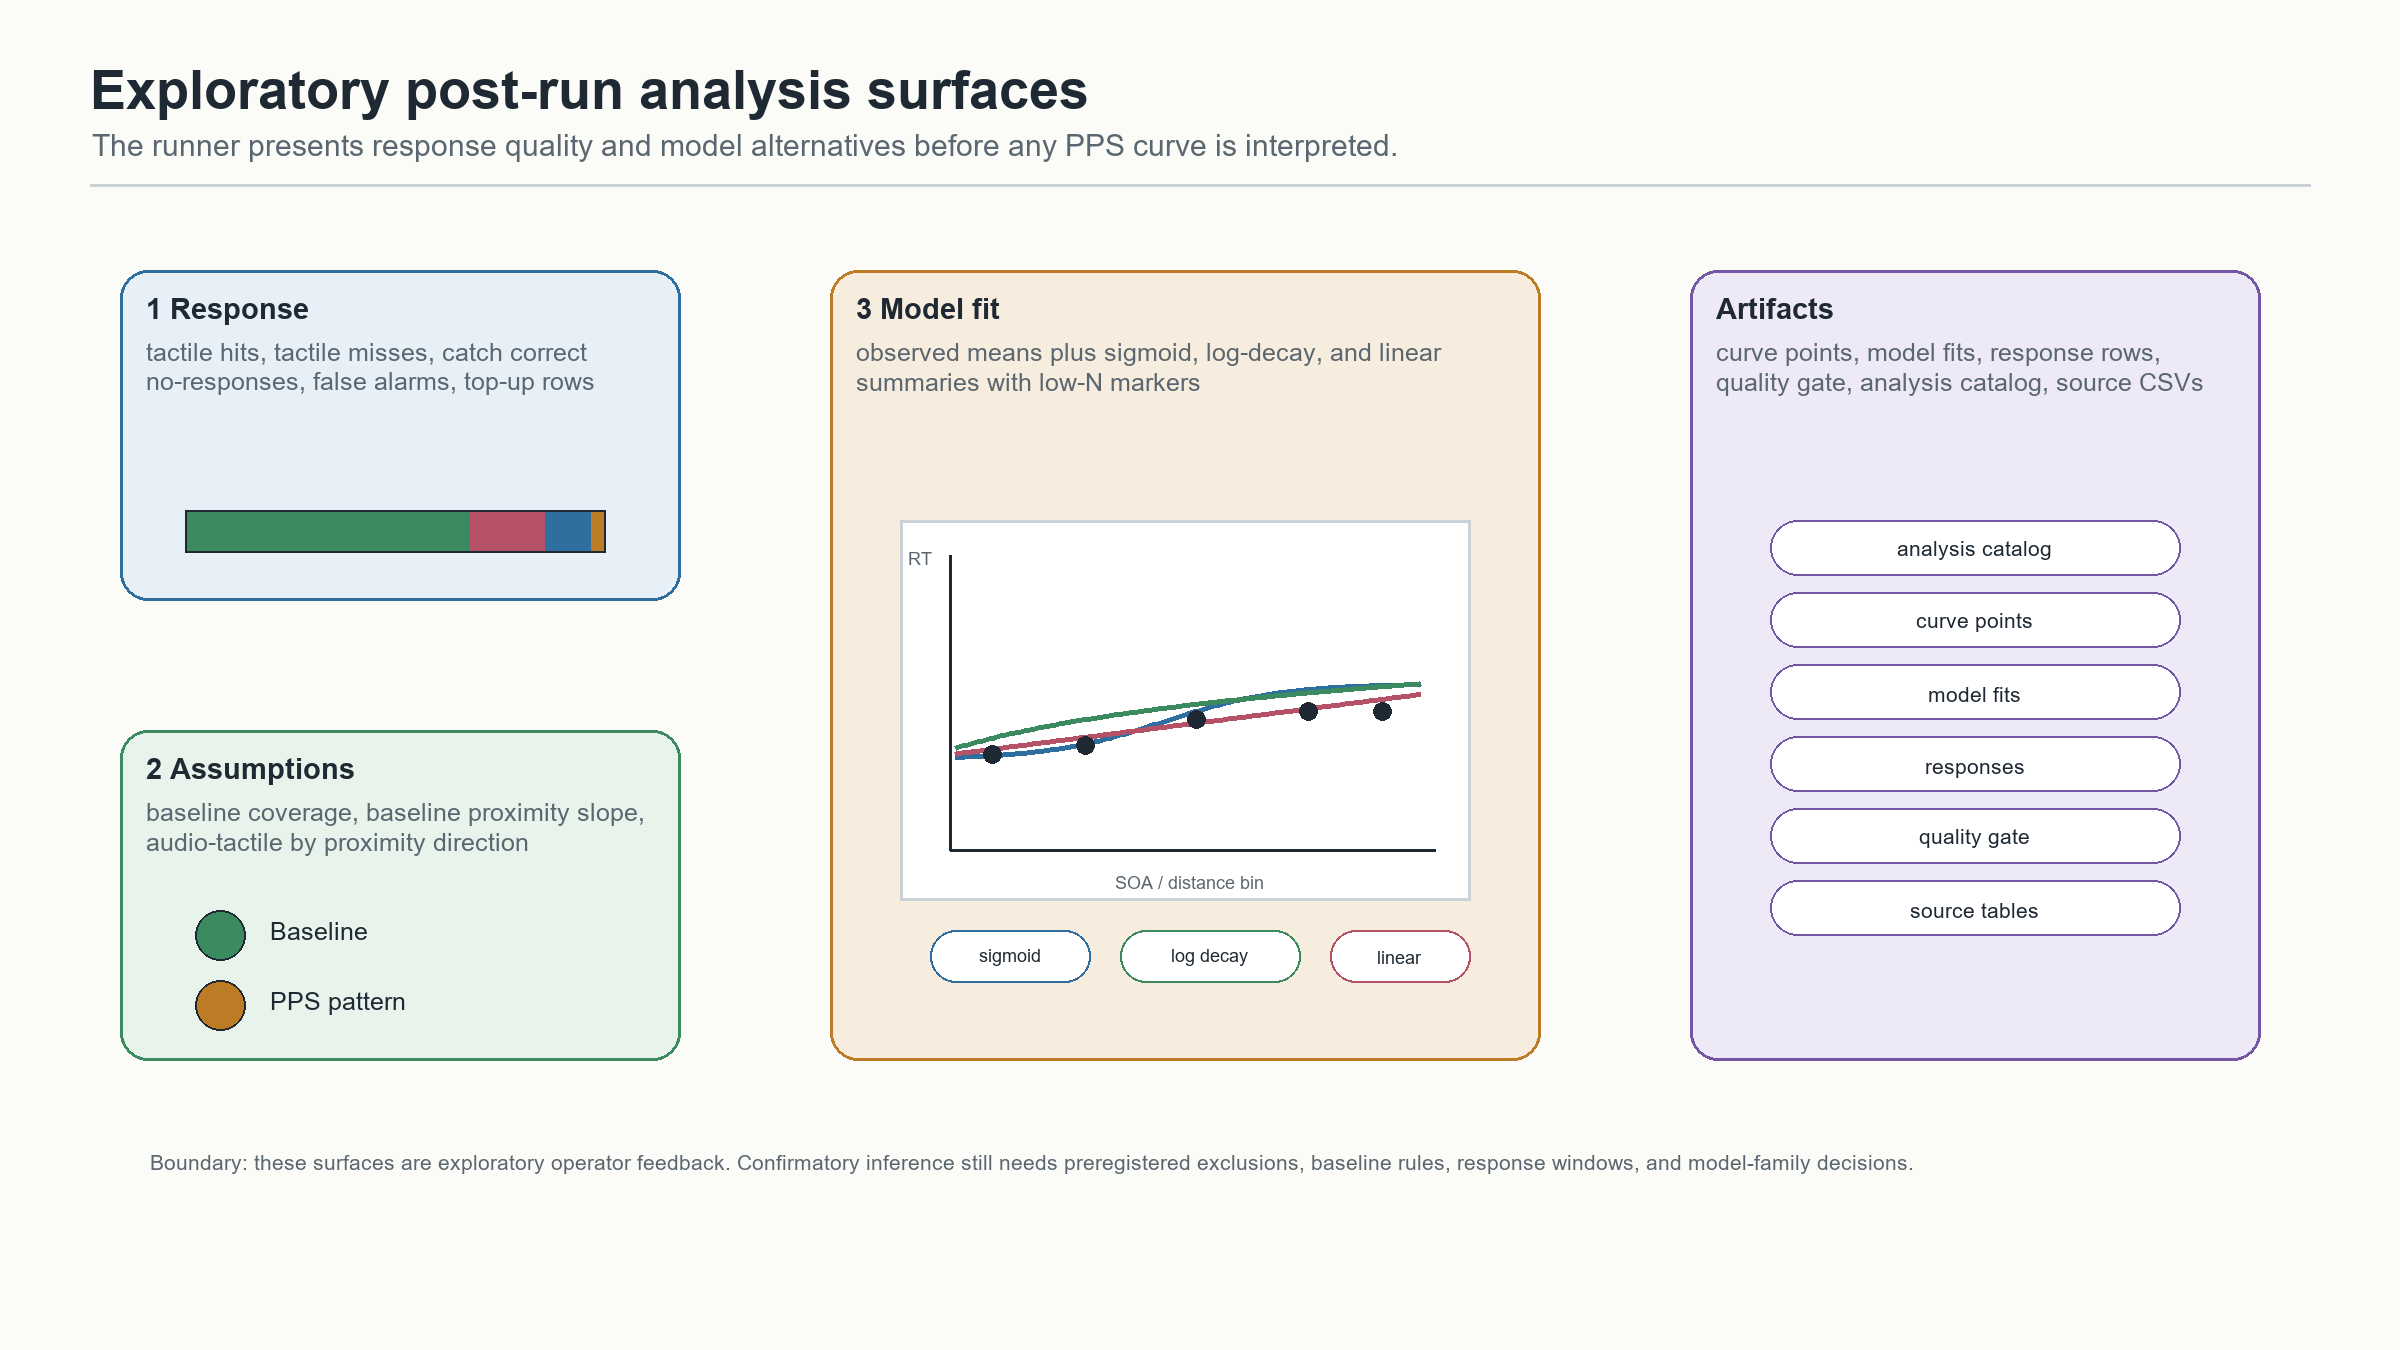
\includegraphics[width=\textwidth]{figures/figure6_analysis_surfaces.png}
\caption{Exploratory post-run analysis surfaces. The schematic summarizes response-quality displays, baseline/PPS assumption checks, model-fit alternatives, low-N cues, and artifact-review outputs. These surfaces are operator feedback and source navigation, not confirmatory PPS inference.}
\label{fig:analysis-surfaces}
\end{figure}

\section{Validation and Use Cases}

We organize validation around four reusable use cases. This draft specifies them as reproducible protocols rather than new participant-level findings. Before submission, the release package must attach the exact run folders, hashes, screenshots, and hardware notes generated for the publication release. The current source-pointer summary sits in \code{validation\_evidence.csv}; Table~\ref{tab:validation} reports the evidence available for this draft without committing the raw generated artifacts.

\begin{table}[t]
\caption{Current validation evidence summarized for the manuscript draft.}
\label{tab:validation}
\footnotesize
\begin{tabularx}{\textwidth}{>{\raggedright\arraybackslash}p{0.22\textwidth} >{\raggedright\arraybackslash}X >{\raggedright\arraybackslash}p{0.22\textwidth} >{\raggedright\arraybackslash}p{0.24\textwidth}}
\toprule
Validation item & Result summary & Evidence layer & Boundary \\
\midrule
Protocol 12 published-profile recreation interface matrix & On 30 June 2026, the scripted matrix passed 30/30 required criteria: seven ready published profiles passed gates and materialized through Segment 6, and two blocked samples were blocked as expected. & Software/profile materialization and runner-handoff artifacts. & Does not prove physical timing, Woojer mechanical onset, tactile perception, individualized spatial perception, or exact reuse of private original-author stimuli. \\
Springer source compile check & The manuscript source compiled with the preserved Springer Nature template with no unresolved citations or references after this revision. & Publication source integrity. & Does not validate runtime behavior or participant-level scientific claims. \\
\bottomrule
\end{tabularx}
\end{table}

\subsection{Study 5-style Workflow}

The first use case runs the bundled \code{study5\_box\_breathing\_pps} profile, which uses local breathing-instruction assets, white and pink frontal burst-train looming sources, stationary-burst baselines, six 34-trial blocks, and runner-owned instruction clips. The validation report walks the chain: Segment 0 activates the profile, Segment 1 materializes the source assets, Segment 2 bakes the inhale/exhale trial families, Segment 3 creates the target, baseline, and catch assets, Segment 4 writes the trial repetition pool, Segment 5 accepts the block CSVs, and Segment 6 prepares the participant package.

\subsection{Published-profile Recreation}

The second use case recreates one published profile, such as \code{canzoneri\_2012\_dynamic\_sounds}, \code{matsuda\_2021\_four\_directions}, or \code{roussel\_2025\_dynaspace\_mobile\_pps}. We do not claim full equivalence to the original apparatus. We show how the toolkit represents the reported timing, the SOA and distance anchors, the direction labels, the baselines, the catch trials, and the missing-parameter caveats.

Table~\ref{tab:profile-families} gives the profile-family map for this use case, and \code{profile\_family\_examples.csv} stores the same rows so a reader can audit the claim outside the PDF. The table stays deliberately conservative: it says what the toolkit can represent procedurally and keeps exact replication conditional on source-paper review, rights clearance, apparatus reconstruction, and local validation.

\begin{table}[t]
\caption{Published-method families represented or scaffolded by PPS Toolkit profiles.}
\label{tab:profile-families}
\footnotesize
\begin{tabularx}{\textwidth}{>{\raggedright\arraybackslash}p{0.18\textwidth} >{\raggedright\arraybackslash}X >{\raggedright\arraybackslash}p{0.27\textwidth}}
\toprule
Profile family & Toolkit representation & Procedural caveat \\
\midrule
Canonical dynamic looming & Dynamic-sounds profiles represent approaching/receding noise-like sources, tactile SOA anchors, control timing, auditory catches, and sigmoid-style summaries from classic audio-tactile PPS work \citep{Canzoneri2012,Farne2002}. & Original apparatus, exact sounds, and participant-level effects remain source-specific. \\
Baseline and expectancy correction & Segment 3 and the analysis layer represent tactile-only, stationary/fixed-distance, auditory-only catch, and baseline-corrected facilitation variants \citep{Hobeika2019,Holmes2020}. & Corrections change the estimand and cannot be treated as a universal repair for fragile or small effects. \\
Directional/body-frame variants & Direction-aware profiles represent front, rear, left, right, and quadrant mappings, plus direction-coupled baselines where reported \citep{Matsuda2021,Teraoka2024,Amiel2025}. & Apparatus geometry, participant-facing direction, and perceived source location must be verified before exact-recreation language is used. \\
Mobile and DynaSpace-style burst trains & Burst-train source metadata, lateral trajectory anchors, fixed comparators, and mobile-profile notes support smartphone/DynaSpace-style recreations \citep{Roussel2025,Hobeika2019}. & Smartphone timing and haptic evidence do not automatically transfer to PC audio-interface, Woojer, or LabRecorder routes. \\
Affective, rough, and ecological sounds & Imported-source profiles preserve source identity, roughness/valence/ecological labels, hashes, and substitution notes \citep{Taffou2021,Ferri2015,Bahadori2021}. & Rights clearance and perceptual equivalence checks are required before redistributing or substituting stimuli. \\
Action, full-body, and immersive variants & Scaffold profiles can store action context, volumetric labels, HRTF/scene metadata, and runner-validation notes for walking or VR-like work \citep{Noel2015,Lerner2021}. & Exact recreation requires locomotion, VR scene, body geometry, spatial rendering, and response apparatus validation. \\
\bottomrule
\end{tabularx}
\end{table}

The family table cannot stand on its own, because a family-level label hides whether a given profile is run-ready, a local example, or a placeholder for a method the current toolkit cannot yet execute faithfully. The source package therefore includes \code{profile\_recreation\_audit.csv}, a per-profile ledger built from \code{assets/preloads/profile\_recreation\_status.json} and each profile's \code{profile\_parameters\_manifest.json}. In the current source state, the ledger sorts 23 preload profiles into two local runnable examples, seven published run-ready profiles, and published scaffolds blocked by missing parameters, unsupported apparatus structures, or both.

\begin{table}[t]
\caption{Per-profile recreation claim states used in the manuscript source package.}
\label{tab:profile-recreation-audit}
\footnotesize
\begin{tabularx}{\textwidth}{>{\raggedright\arraybackslash}p{0.18\textwidth} >{\raggedright\arraybackslash}p{0.28\textwidth} >{\raggedright\arraybackslash}X >{\raggedright\arraybackslash}p{0.23\textwidth}}
\toprule
Audit class & Examples in current ledger & Allowed claim & Claim boundary \\
\midrule
Published verified run-ready & Roussel/DynaSpace mobile, Matsuda four-direction, Barumerli arm-movement, Noel bodily-self, and Pfeiffer lateral peri-head profiles. & The profile represents encoded source, trajectory, SOA, tactile, baseline/catch, repetition, and runner-handoff fields and can materialize through Segment 6. & It is still not proof of original hardware, participant perception, unpublished source assets, or participant-level effects. \\
Partial but materializable & \code{serino\_2015\_peri\_trunk\_exp1}. & The current GUI can run the encoded audio-tactile scaffold, and Protocol 12-style materialization can test the handoff. & The partial-source-audit caveat remains until the remaining apparatus/source checks are closed. \\
Unpublished local examples & \code{study5\_box\_breathing\_pps} and \code{study5\_dynaspace\_lateral\_45\_pps}. & These profiles demonstrate the suite workflow for design, materialization, runner handoff, and validation-layer reporting. & They are not published-study recreations and are not literature replication evidence. \\
Missing-parameter scaffolds & Tool-use, amputation/prosthesis, Ferri affective/ecological, walking, synchronous-training, and social-face examples. & The profile records a source-paper pointer and the fields currently known or approximated. & The profile is not recreation-ready until missing trial counts, timing tables, gain envelopes, tactile calibration, response-capture, or rights fields are encoded. \\
Structural-gap scaffolds & Canonical Canzoneri dynamic-sounds, echolocation, wheelchair, 3D/VR, front/back speaker-array, peri-hand coordinate, and rear/threat examples. & The profile is useful for identifying the method family and the toolkit feature gap. & Exact recreation requires new toolkit support or a validated approximation for speaker arrays, body-scaled 3D rendering, direction-coupled baselines, lateral hand frames, rear hemifields, or HRTF/source rights. \\
\bottomrule
\end{tabularx}
\end{table}

\subsection{Timing and Output Evidence}

The third use case demonstrates the evidence-tier distinction. A software-only run verifies the manifest-to-event-log reconstruction. A digital audio evidence WAV verifies the mixed sample content. An electrical loopback route estimates audio-interface skew or trigger visibility when loopback hardware is connected. A tactile threshold report documents the perceptual preset. None of these collapse into a single timing claim. A publishable report states which tiers ran on the publication hardware and which remain unvalidated.

\subsection{Pre-run Qualification Checklist}

The design archive and runner package are necessary but not sufficient for a publication-grade participant session. Before data collection, a laboratory still has to qualify the participant, the listening route, the tactile route, the timing route, and the analysis plan that will carry its strongest claim. This separation follows the same logic as headphone and listening checks, web psychoacoustics validation, timing mega-studies, mobile tactile-timing work, and the PPS baseline critiques \citep{Milne2021,Mok2023,Bridges2020,Hirst2026,Roussel2025,Holmes2020,Hobeika2019}.

Table~\ref{tab:pre-run-checklist} turns the procedural gap register into a pre-run checklist. The full source ledger, with per-row citation keys and Consensus URLs, sits in \code{pre\_run\_qualification\_checklist.csv}.

\begin{table}[t]
\caption{Pre-run qualification checklist for publication examples.}
\label{tab:pre-run-checklist}
\footnotesize
\setlength{\tabcolsep}{3pt}
\begin{tabularx}{\textwidth}{>{\raggedright\arraybackslash}p{0.18\textwidth} >{\raggedright\arraybackslash}X >{\raggedright\arraybackslash}p{0.26\textwidth} >{\raggedright\arraybackslash}p{0.22\textwidth}}
\toprule
Layer & Record before data collection & Toolkit evidence already available & Boundary \\
\midrule
Listening eligibility & Hearing or hearing-screen policy, headphone/transducer check, room notes, level setting, and whether SPL is measured or estimated. & Route settings, output checks, and loudness-policy manifests. & Playback success is not normal hearing, headphone compliance, externalization, or ear-level SPL evidence. \\
Spatial rendering and perception & SOFA/HRTF resource, renderer, trajectory frame, level law, and any localization or externalization check. & Renderer manifests, source hashes, channel maps, and trajectory ledgers. & HRTF provenance is stimulus provenance, not perceived-space proof. \\
Route timing and synchronization & Operating system, runner version, audio interface, channel map, buffer settings, response device, LSL/LabRecorder state, loopback wiring, and reconciliation hashes. & Software events, LSL mirrors, optional XDF, audio evidence WAVs, and optional loopback files. & Software markers do not prove physical sound, tactile onset, or response-device latency. \\
Tactile readiness & Actuator, body site, threshold assay, accepted output value, confirmation counters, misses, top-up policy, adaptive-threshold settings, and mechanical or perceptual evidence when claimed. & Threshold reports, miss/top-up ledgers, and adaptive-threshold CSV/JSON artifacts. & Safeguards do not prove habituation correction or mechanical/perceived tactile delivery. \\
Task and response governance & Baseline strategy, catch trials, repetitions, block order, response window, planned cell counts, and confirmatory versus exploratory analysis status. & Segment 3--6 manifests, block CSVs, response rules, and instant-analysis outputs. & A balanced schedule or curve does not remove expectancy, response-probability, or flexible-analysis confounds. \\
Profile provenance and rights & Source-paper status, missing parameters, substitutions, stimulus rights, final profile hash, and exact/partial/scaffold claim state. & Profile family and recreation-audit ledgers, source pointers, hashes, and materialization status. & A runnable profile can still be a scaffold. \\
\bottomrule
\end{tabularx}
\end{table}

\subsection{Operator Procedure and Evidence Handoff}

A publishable participant session extends the Segments 0--6 design workflow into operator actions, and each action produces a bounded evidence object. Table~\ref{tab:operator-procedure} gives the compact procedure, both for the publication example and for a laboratory adapting the toolkit.

\begin{table}[t]
\caption{Operator procedure and evidence handoff for a publishable PPS Toolkit run.}
\label{tab:operator-procedure}
\footnotesize
\begin{tabularx}{\textwidth}{>{\raggedright\arraybackslash}p{0.16\textwidth} >{\raggedright\arraybackslash}X >{\raggedright\arraybackslash}p{0.25\textwidth} >{\raggedright\arraybackslash}p{0.22\textwidth}}
\toprule
Stage & Operator action & Written evidence & Boundary \\
\midrule
Pre-run setup & Select profile/package, participant code, part order, output route, response target, loopback, LabRecorder, and top-up settings before playback is enabled. & Setup metadata, copied profile snapshot, route settings, package manifest, and optional capture configuration. & Confirms intended administration, not physical timing or perception. \\
Output and calibration & Run audio/tactile checks; complete the participant tactile-threshold assay when used; keep accepted calibration separate from trial rows. & Tactile calibration JSON/CSV/report, output settings, route notes, and threshold confirmation counters. & A perceptual preset is not a mechanical actuator-onset measurement. \\
Execution & Present instructions, start blocks, preserve deterministic block order, log clicks, markers, pauses, recenter actions, misses, adaptive-threshold events, and top-up decisions. & Participant CSV rows, event logs, LSL mirrors, LabRecorder/XDF files when enabled, top-up ledgers, adaptive-threshold artifacts, and audio evidence WAVs when enabled. & Software and electrical evidence must be interpreted by tier; top-up rows do not erase original misses. \\
Post-run review & Inspect completion status, response quality, baseline coverage, low-N warnings, timing evidence, and exploratory model fits before sharing deidentified outputs. & Analysis catalog, response summaries, assumption checks, model-fit tables, validation reports, and archive manifests. & Instant analysis is operator feedback unless a preregistered confirmatory analysis is supplied. \\
Sharing & Publish design/profile, validation, and deidentified participant layers separately with hashes and rights notes. & Release tag or DOI, source commit, design archive, validation archive, data dictionary, and materials availability statement. & Copyrighted stimuli, private outputs, local SOFA files, and proprietary vendor tools stay outside the public license unless rights are explicit. \\
\bottomrule
\end{tabularx}
\end{table}

\subsection{Procedural Gap Register}

The suite also states what it does not yet solve. This is not a failure of the method but a BRM-style evidence boundary: timing-sensitive and sensory tool papers routinely separate what the software can schedule from what a route, device, participant, or analysis plan has actually validated \citep{Bridges2020,Reimers2016,Garaizar2019,Hirst2026}. Table~\ref{tab:gap-register} lists the procedural gaps that a release must either close in the example or keep as explicit caveats. The same register sits in \code{procedural\_gap\_register.csv}.

\begin{table}[t]
\caption{Procedural gaps to close or explicitly caveat before submission.}
\label{tab:gap-register}
\footnotesize
\begin{tabularx}{\textwidth}{>{\raggedright\arraybackslash}p{0.17\textwidth} >{\raggedright\arraybackslash}X >{\raggedright\arraybackslash}p{0.28\textwidth} >{\raggedright\arraybackslash}p{0.22\textwidth}}
\toprule
Gap & Toolkit coverage & Publication-ready addition & Boundary \\
\midrule
Auditory eligibility & The runner records route settings and output checks. & Add hearing/headphone/listening-room screening and sound-level measurement or level-setting artifacts \citep{Mok2023,Milne2021}. & Route selection is not hearing, headphone, externalization, or ear-level SPL evidence. \\
Route timing & The toolkit writes software schedules, event logs, audio evidence, LSL/XDF mirrors, and optional loopback reports. & Attach a publication-hardware archive with route diagram, channel map, response-device check, loopback method, reconciliation report, and hashes \citep{Bridges2020,Reimers2016,Garaizar2019,Pronk2020}. & Software markers do not prove physical output onset or response latency. \\
Tactile delivery & Focus Mode has threshold calibration, miss logging, top-up, and the two-miss adaptive nudge. & Add calibration examples, adaptive-threshold ledgers, and mechanical/electrical timing evidence where available \citep{Hirst2026,Merchel2020,Mikkelsen2020,Goble1993,Pate2024}. & The adaptive nudge is a safeguard, not a validated habituation correction. \\
Spatial perception & Renderer manifests record SOFA/HRTF resource, trajectory, channel layout, hashes, and loudness policy. & Add localization, externalization, individualized-HRTF, or spatial-route screening evidence for any strong spatial claim \citep{CuevasRodriguez2019,Salvador2018,Parseihian2014,Kan2009,Spagnol2017}. & HRTF provenance is not participant-level perceived-distance evidence. \\
Recreation and analysis governance & Profiles record represented fields, missing fields, substitutions, baselines, response rules, and exploratory model choices. & Before exact-recreation or empirical claims, attach profile source audits, rights ledger, archived hashes, data dictionary, and preregistered analysis choices \citep{Holmes2020,DeLeeuw2022,Ellis2024}. & A runnable scaffold is not an exact apparatus or confirmatory-analysis replication. \\
\bottomrule
\end{tabularx}
\end{table}

\subsection{Post-run Analysis Review}

The fourth use case loads a completed sample or deidentified run and shows the instant-analysis outputs: response integrity, the baseline assumption, the PPS assumption, the model-fit families, low-N warnings, and artifact paths. The validation criterion is not that the sample yields a strong PPS effect. It is that the analysis labels its own limits, preserves the baseline metadata, and keeps exploratory operator feedback from hardening into a hidden confirmatory pipeline.

\subsection{Figure and Source-material Plan}

A reviewer evaluates a BRM software paper more easily when the figures show both the tool workflow and the evidence boundary. This draft therefore includes six source-owned schematic figures, generated by \code{figures/generate\_figures.py}. They are redistributable manuscript assets, not screenshots from private participant sessions or figures copied from source papers.

Table~\ref{tab:figure-plan} lists the current schematic figure set, the tracked source artifact behind each figure, and the claim boundary. Release-state dashboard screenshots, validation-output plots, or deidentified sample-analysis figures can replace or supplement these schematics later, archived with their exact source files and hashes. The same plan sits in \code{figure\_source\_plan.csv}.

\begin{table}[!htbp]
\caption{Current schematic figure source map and claim boundaries.}
\label{tab:figure-plan}
\footnotesize
\setlength{\tabcolsep}{3pt}
\begin{tabularx}{\textwidth}{>{\raggedright\arraybackslash}p{0.18\textwidth} >{\raggedright\arraybackslash}p{0.42\textwidth} >{\raggedright\arraybackslash}X}
\toprule
Figure & Source basis & Boundary \\
\midrule
Workflow & Generated schematic from \code{generate\_figures.py}; exact path in \code{figure\_source\_plan.csv}. & Workflow evidence, not timing or behavioral validation. \\
Design matrix & Generated schematic backed by the evidence matrix, GUI-control ledger, and profile-family map. & Structured evidence map, not PRISMA/meta-analysis. \\
Stimulus choices & Generated schematic backed by source-mode, trajectory, and baseline/catch manifests. & Does not prove perceptual equivalence to private original stimuli. \\
Evidence tiers & Generated schematic backed by renderer, route, event, and validation ledgers. & Does not prove individualized localization or tactile mechanical onset. \\
Operator safeguards & Generated schematic backed by calibration, adaptive-threshold, top-up, and operator-procedure schemas. & Safeguard documentation, not proof of habituation correction. \\
Exploratory analysis & Generated schematic backed by instant-analysis CSV/JSON schemas and source ledgers. & Exploratory review, not confirmatory PPS inference. \\
\bottomrule
\end{tabularx}
\end{table}

\section{Discussion}

\toolkit{} attacks a recurring problem in audio-tactile PPS research: the design differences that carry theoretical weight are exactly the ones the implementing software tends to hide. The toolkit does not flatten the field into one standard paradigm. It makes the heterogeneity explicit.

A researcher can pick burst-train or smooth looming sources, front or rear trajectories, tactile-only or stationary baselines, a one-part or pre/post schedule, and a sigmoid or graded model summary. The binding constraint is that each choice becomes a manifest entry, a CSV row, a hash, or a caveat instead of an undocumented runtime assumption.

The evidence matrix also marks where the toolkit is mature and where it remains a scaffold. It already runs the core dynamic audio-tactile PPS family: generated or imported looming audio, SOA-based tactile insertion, baseline and catch assets, deterministic block review, native runner preparation, event and LSL mirrors, optional LabRecorder capture, and exploratory analysis.

It only partly represents paradigms that hinge on licensed emotional sounds, social contexts, walking or wheelchair tasks, analog speaker arrays, detailed VR scenes, individualized HRTFs, or body-part-specific apparatus geometry. There the profile gives a structured starting point, but it is not an exact replication until someone resolves the missing fields.

The tactile-threshold workflow shows the same philosophy. Calibrating tactile output is worth doing because vibrotactile thresholds vary across participants and methods \citep{Merchel2020,Mikkelsen2020,Pate2024}. Yet near-threshold calibration can raise misses over a long task, and adaptation can shift detection thresholds \citep{Goble1993,Hollins1990}. We document the two-miss nudge as a safeguard with its own artifacts, not as a confirmed correction, and future validation has to test whether the rule improves response completeness without introducing condition-dependent bias.

The paper positions \toolkit{} as a methods instrument, not a theory adjudicator. Whether a given experiment supports a sharp boundary, a graded log-distance function, a direction-specific defensive asymmetry, or no reliable PPS effect stays an empirical question. The toolkit's job is to make the experiment explicit enough that the field can evaluate such a claim.

\section{Limitations and Future Work}

Several tasks remain before submission. We must complete the author affiliations, funding, ethics statements, repository URLs, release DOI, and final license wording. We must summarize at least one publication-hardware validation report with exact tool versions and artifact hashes. We must back any tactile hit-rate or adaptation claim with traceable run artifacts or drop it. We must restrict exact profile-recreation claims to profiles whose original methods, supplements, and assets we have checked. And we must generate every figure in the final submission from redistributable toolkit artifacts, not from copyrighted papers or private participant data.

\section{Conclusion}

An audio-tactile PPS experiment needs both flexibility and provenance. \toolkit{} delivers a segmented design-run-recreation workflow that exposes the decisions studies differ on, stores them as reusable artifacts, and keeps software, electrical, and perceptual evidence apart. That combination makes it a Behavior Research Methods contribution: a practical, open, auditable method for building, running, and recreating PPS experiments without forcing the field's diversity into a single mold.

\section*{Declarations}

\subsection*{Code availability}
We intend to release the PPS Toolkit source code in the project's public GitHub repository under the repository license. Before submission, this section must give the release tag, the archived DOI if available, the installation instructions, and the exact commit used for the paper.

\subsection*{Data availability}
This manuscript draft reports no new participant dataset. If the submitted manuscript includes deidentified sample data, we will list it with its repository paths and sharing terms. Raw participant outputs, local generated artifacts, and private acquisition folders stay outside the public repository unless we separately deidentify and approve them for release.

\subsection*{Materials availability}
The repository stores the redistributable toolkit materials, study templates, generated-source parameters, and manifest examples. We do not redistribute third-party SOFA/HRIR files, vendor software, copyrighted papers, proprietary sounds, or private participant outputs unless we have verified their rights.

\subsection*{Ethics approval and consent to participate}
This methods and software manuscript draft reports no new human-subject data. Any final manuscript that adds participant validation or pilot data must include the relevant ethics approval, consent, and data-sharing language.

\subsection*{Competing interests}
To be completed before submission. The draft currently assumes no competing interests.

\subsection*{Funding}
To be completed before submission.

\subsection*{Author contributions}
To be completed before submission.

\section*{Open Practices Statement}
This draft reports software and reusable methods rather than a new participant experiment, and it analyzes no new participant dataset. We intend to share the manuscript source, the evidence matrix, the validation-evidence summary, the study-template source pointers, and the toolkit code in the public repository, adding the final release tag, archived DOI, and exact paper commit before submission. We do not commit generated local validation reports, participant folders, raw downloaded papers, proprietary sounds, or private acquisition outputs. Any final version that reports participant or hardware-validation results must archive the redistributable validation artifacts, hashes, analysis scripts, and deidentified data needed to reproduce those claims.

\bibliography{references}

\end{document}
